\section{并发/并行/异步}
Rust也同样支持常见的并行和并发操作,也同样分为进程,线程以及消息通信等等。

\subsection{线程}
Rust的线程操作必须使用闭包完成。在之前看到的闭包当中,通常采用的都是有参的闭包,
而在Rust的线程操作当中,则经常会遇到无参数的闭包;Rust的线程使用thread::spawn函数
进行实现:
\begin{code-block}{rust}
use std::thread;
use std::time::Duration;
fn main() {
    thread::spawn(|| {
        for i in 1..10 {
            println!("hi number {} from the spawned thread!", i);
            thread::sleep(Duration::from_millis(1));
        }
    });
    for i in 1..5 {
        println!("hi number {} from the main thread!", i);
        thread::sleep(Duration::from_millis(1));
    }
}
\end{code-block}
和其他语言的线程概念一样,当主线程结束时,所有的线程都会被终止。因此上述代码当中,
子线程(spawn)无法将所有的循环执行完成。为了达成所有进/线程执行完成之后才退出主
进/线程的目的,和其他的开发语言相同,需要在主进程当中调用join函数:
\begin{code-block}{rust}
fn main() {
    let handle = thread::spawn(|| {
        for i in 1..10 {
            println!("hi number {} from the spawned thread!", i);
            thread::sleep(Duration::from_millis(1));
        }
    });
    for i in 1..5 {
        println!("hi number {} from the main thread!", i);
        thread::sleep(Duration::from_millis(1));
    }
    handle.join().unwrap();
}
\end{code-block}
Thread::spawn的返回值是JoinHandle,是一个拥有所有权的值,当对其调用join方法时,
它会等待对应线程结束;而join的返回值是一个Result,可以按照之前介绍的方式进行处理。
同时,Join函数是一个阻塞式函数,只有当该函数运行结束之后,才会继续进行后续的操作。

多数情况下,Rust的线程不可能只会在内部运行,而和外部没有数据交互。但是,如果我们
直接使用外部数据,则会出现错误,比如下方的代码:
\begin{code-block}{rust}
fn main() {
    let v = vec![1, 2, 3];
    let handle = thread::spawn(|| {
        println!("Here's a vector: {:?}", v);
    });
    handle.join().unwrap();
}
\end{code-block}
\begin{figure}[H]
  \centering
  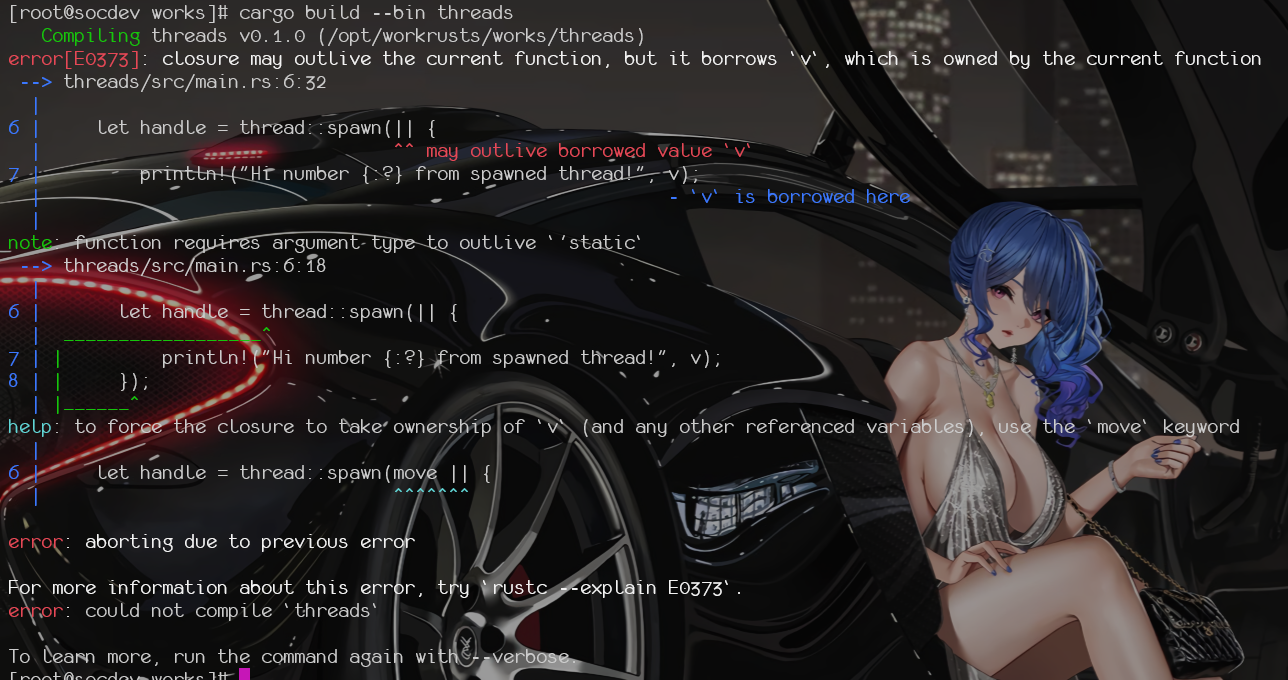
\includegraphics[width=\linewidth]{rust_thread_out_params.png}
  \caption{试图访问线程外部资源}
  \label{fig:rust_thread_out_params}
\end{figure}
线程使用的是闭包,从闭包的定义来说,是可以捕获并使用外部变量和数据的;但是,Rust
不知道这个线程到底会运行多长时间,因此无法知道对外部变量的引用是否一直有效,比如
下方的代码:
\begin{code-block}{rust}
fn main() {
    let v = vec![1, 2, 3];
    let handle = thread::spawn(|| {
        println!("Here's a vector: {:?}", v);
    });
    drop(v);
    handle.join().unwrap();
}
\end{code-block}
启动线程的同时,立即将v进行丢弃,线程内部无法知道v在运行阶段是否继续有效,就会
出现错误,因此,如果在线程当中使用默认的闭包模式,则无法对应的闭包是无法捕获以及
使用外部的变量和数据的。此时,则需要使用move闭包进行替换,即强制闭包获取外部变量
的所有权,而不是由Rust进行借用推断。但是需要注意,一旦使用move之后,在线程之外,
变量将无法再进行使用:
\begin{code-block}{rust}
fn main() {
    let v = vec![1, 2, 3];
    let handle = thread::spawn(move || {
        println!("Here's a vector: {:?}", v);
    });
    // 下方代码无法再进行执行
    // println!("{:?}", v);
    handle.join().unwrap();
}
\end{code-block}

\subsection{消息通信和消息传递}
每个线程做自己的事情,但是,不管什么编程语言,都需要考虑线程之间的数据交互问题。
Rust向Golang进行了学习,使用通信替换共享内存,来进行线程之间的数据传输。同样的,
Rust当中用于消息传递并发的主要工具是通道,该概念和Golang的通道概念相同。Rust的通道
分为2个角色:发送者和接收者,发送者发送消息,接收者接收消息,当发送者或者接收者任一
被丢弃时,则对应的通道被视为关闭。

Rust的通道采用mpsc::channel函数实现,mpsc表示多个生产者,单个消费者,因此,Rust
标准库实现通道的方式意味着一个通道可以有多个产生值的发送(sending)端,但只能有
一个消费这些值的接收(receiving)端。通道的实现示例如下:
\begin{code-block}{rust}
use std::sync::mpsc;
fn main() {
    let (sender, recevier) = mpsc::channel();
}
\end{code-block}
其中,函数的第一个返回值为发送者,第二个参数为接收者。使用通道发送数据通信的示例
如下:
\begin{code-block}{rust}
use std::sync::mpsc;
use std::thread;
fn main() {
    let (sender, recevier) = mpsc::channel();
    thread::spawn(move || {
        let val = "lucifer".to_string();
        match sender.send(val) {
            Ok(_) => println!("Send success"),
            Err(error) => println!("Send failed :{:?}", error),
        }
    });
    let res = match recevier.recv() {
        Ok(s) => s,
        Err(error) => {
            println!("Cannot recevie anything from sender: {:?}", error);
            "".to_string()
        }
    };
    println!("The result of channel is {}", res);
}
\end{code-block}
接收者接收消息有2种模式:默认的recv是阻塞式,返回一个Result<T, E>,当通道关闭时,
将返回Result当中的Error;而try\_recv是非阻塞式,同样是返回一个Result<T, E>,但是,
Result当中的Error表示没有接收到任何消息,可以使用for循环进行反复的尝试读取操作。
另外需要注意的是,Send函数会改变变量的所有权,当该函数执行之后,被发送的消息
(变量)将无法再使用。

但是,通道可以反复使用,而且和Golang的类似,Rust的通道也是可以进行迭代的,特别
是在接收消息时,通常采用for循环进行操作,减少了错误处理的代码,使得代码更具可读性:
\begin{code-block}{rust}
use std::sync::mpsc;
use std::thread;
fn main() {
    let (sender, recevier) = mpsc::channel();

    let handler = thread::spawn(move || {
        let vals = vec!["lucifer", "titans", "garuda"];
        for val in vals {
            match sender.send(val) {
                Ok(_) => println!("Send success"),
                Err(error) => println!("Send failed :{:?}", error),
            }
        }
    });
    for msg in recevier {
        println!("The msg is {}", msg);
    }
    match handler.join() {
        Err(error) => println!("Error{:?}", error),
        _ => (),
    }
}
\end{code-block}

同样的,由于Rust的通道默认是多生产者/单消费者,因此,可以通过多个发送端向单个接
收端发送消息。实际使用当中的多个发送端,则通常是某个发送端的克隆对象,如下:
\begin{code-block}{rust}
use std::sync::mpsc;
use std::thread;
fn main() {
    let (sender, recevier) = mpsc::channel();
    let sender_copy = sender.clone();

    let handler = thread::spawn(move || {
        let vals = vec!["lucifer", "titans", "garuda"];
        for val in vals {
            match sender.send(val) {
                Ok(_) => println!("Send success"),
                Err(error) => println!("Send failed :{:?}", error),
            }
        }
    });
    let handler_copy = thread::spawn(move || {
        let vals = vec!["zhangjl", "luoyan", "zhangzz"];
        for val in vals {
            match sender_copy.send(val) {
                Err(error) => println!("Send failed :{:?}", error),
                _ => (),
            }
        }
    });
    for msg in recevier {
        println!("The msg is {}", msg);
    }
    match handler_copy.join() {
        Err(error) => println!("Error{:?}", error),
        _ => (),
    }
    match handler.join() {
        Err(error) => println!("Error{:?}", error),
        _ => (),
    }
}
\end{code-block}

\subsection{共享状态}
在其他语言当中,有些特殊的场景,还是必须使用原有的线程并发概念——锁——来进行资源的
访问/读写控制。Rust当中同样存在锁,比较常见的就是互斥锁(互斥器,Mutex)以及原子
计数器(Arc)。在基本的操作上,互斥锁的使用和其他语言当中没有太大的区别:
\begin{code-block}{rust}
use std::sync::Mutex;
fn main() {
    let m = Mutex::new(5);
    {
        let mut num = m.lock().unwrap();
        *num = 6;
    }
    println!("m = {:?}", m);
}
\end{code-block}
注意,上述代码如果将内部大括号去除,则运行结束之后,m的状态还是锁定状态;但是,
有大括号,则表示大括号内部的段是一个有效的生命周期,当该生命周期结束之后,互斥
锁将自动释放。一旦获取了锁,就可以将返回值(在这里是num)视为一个其内部数据的
\colorblock{可变引用}。类型系统确保了我们在使用m中的值之前
获取锁:Mutex<i32>并不是一个i32,所以必须获取锁才能使用这个i32值。

实质上,Mutex是一个智能指针,lock调用返回一个叫做MutexGuard的智能指针。这个智能
指针实现了Deref来指向其内部数据;同时也提供了一个Drop实现,使得MutexGuard离开作
用域时自动释放锁,即锁的释放是自动发生的。

但是默认情况下,Mutex是无法用于进行线程间的数据共享,如下:
\begin{code-block}{rust}
use std::rc::Rc;
use std::sync::Mutex;
use std::thread;
fn main() {
    let counter = Rc::new(Mutex::new(0));
    let mut handles = vec![];
    for _ in 0..10 {
        let counter = Rc::clone(&counter);
        let handle = thread::spawn(move || {
            let mut num = counter.lock().unwrap();
            *num += 1;
        });
        handles.push(handle);
    }
    for handle in handles {
        handle.join().unwrap();
    }
    println!("Result: {}", *counter.lock().unwrap());
}
\end{code-block}
上述代码会出现下面的类似错误:
\begin{figure}[H]
  \centering
  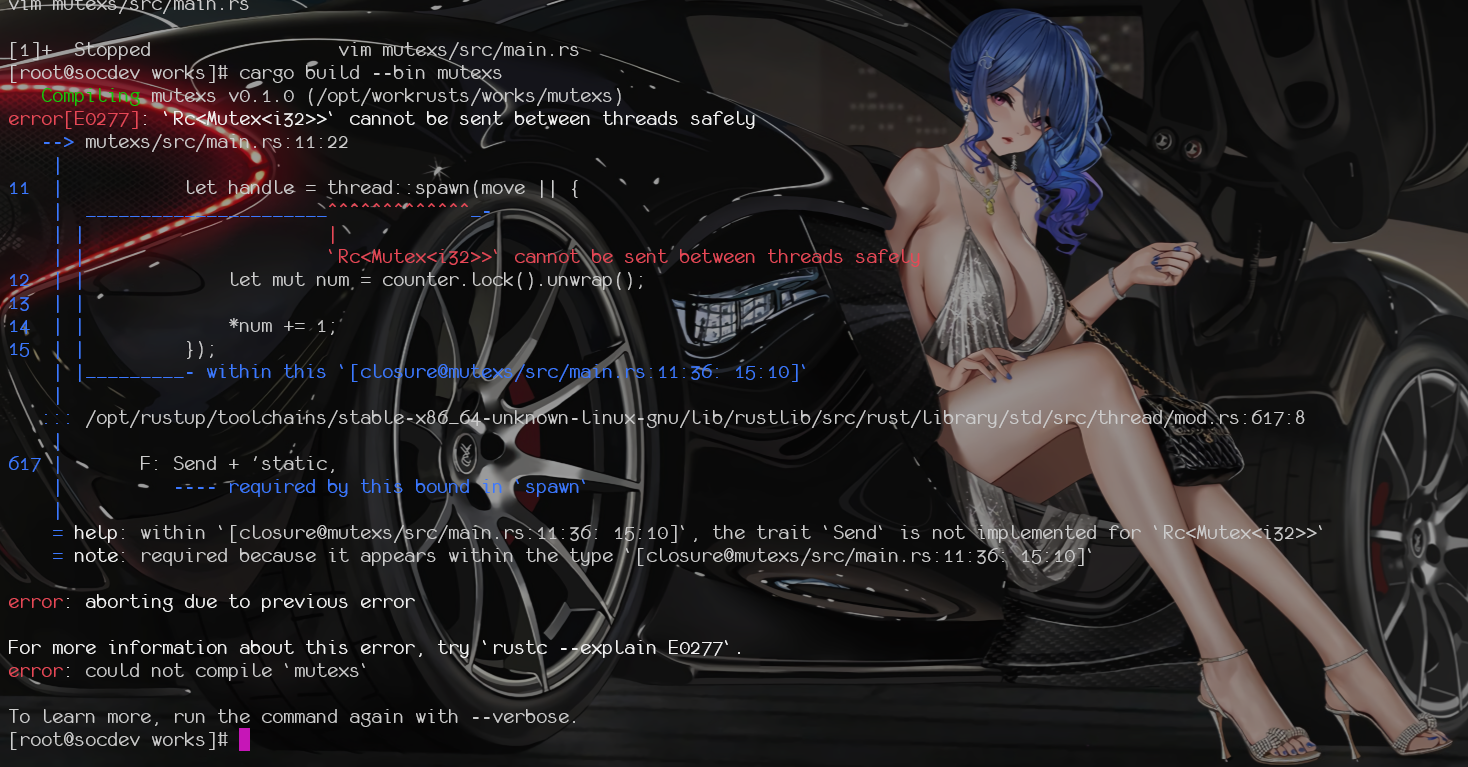
\includegraphics[width=\linewidth]{rust_mutex_share_error.png}
  \caption{试图通过Rc共享Mutex的数据}
  \label{fig:rust_mutex_share_error}
\end{figure}
即之前提到的,Rc类型只能用于单线程/单进程环境。

而共享引用计数则需要使用Arc,它是可以安全的用于并发环境的类型,即原子引用计数,
可以在线程间进行共享所有权。Arc和Rc有相同的API,基本使用方法上类似。所有,可以直
接对上述代码进行修改:
\begin{code-block}{rust}
use std::sync::{Arc, Mutex};
use std::thread;
fn main() {
    let counter = Arc::new(Mutex::new(0));
    let mut handles = vec![];
    for _ in 0..10 {
        let counter = Arc::clone(&counter);
        let handle = thread::spawn(move || {
            let mut num = counter.lock().unwrap();
            *num += 1;
        });
        handles.push(handle);
    }
    for handle in handles {
        handle.join().unwrap();
    }
    println!("Result: {}", *counter.lock().unwrap());
}
\end{code-block}
通过这样简单的修改,成功实现了10个进程当中对同一个数值进行加法操作的功能。

虽然Rust本身的线程/进程管理非常完善,但是,thread::spawn产生的线程没有名称,并且
其栈空间大小默认为2M,如果需要需要针对线程/进程进行粒度更细的操作,比如自定义
线程名称,自定义线程的资源等等,此时,就需要使用thread::Builder进行修改,具体示例
如下:
\begin{code-block}{rust}
let mut v_thread = vec![];
for id in 1..5 {
    let thread_name = format!("child-{}", id);
    let size: usize = 1024;
    // 定义线程的名称,设置线程占用的栈大小为1M(1024)
    let builder = Builder::new().name(thread_name).stack_size(size);
    // builder.spawn返回的是Result<JoinHander, std::io::Error>
    // 需要进行处理,取出真正的线程句柄
    match builder.spawn(move || {
        info!(
            "In the child: {}, and the child name is {}",
            id,
            current().name().unwrap()
        );
    }) {
        Ok(child) => v_thread.push(child),
        Err(error) => error!("Cannot create the thread {} because: {:?}", id, error),
    };
}
// 其他的同普通的线程,
for child in v_thread {
    child.join().unwrap();
}
\end{code-block}

由于线程包含自己的资源空间,因此,存在一个特殊的存储空间——线程本地存储(Thread Local Storage,TLS),
存放在该区域的资源,其他线程无法访问,而是每个线程独占的数据:
\begin{code-block}{rust}
use std::cell::RefCell;
use std::thread;
fn main() {
    // 在线程本地存储定义一个FOO变量,最终的类型是thread::LocalKey
    thread_local!(static FOO: RefCell<u32> = RefCell::new(1));
    // 提供了一个with方法,可以通过给该方法传入闭包
    // 来操作线程本地存储中包含的变量
    FOO.with(|f| {
        info!("The f borrow is {}", *f.borrow());
        *f.borrow_mut() = 2;
    });
    let handler = thread::spawn(move || {
        // 子线程也有一个线程本地存储实例FOO,为主线程的副本
        // 也可以使用thread_local!宏在该子线程中重新创建一个LocalKey实例
        FOO.with(|f| {
            info!("In the handler thread The f borrow is {}", *f.borrow());
            *f.borrow_mut() = 3;
        });
    });
    // 主线程当中FOO实例并没有被子线程修改为3
    // thread local!宏定义单个线程内的一些独享数据
    FOO.with(|f| {
        info!("The f borrow is {}", *f.borrow());
    });
    handler.join().unwrap();
}
\end{code-block}

在同步原语支持方面,Rust也有自己的实现方式,通过使用std::thread当中的park函数提供
阻塞线程的能力,但并不能永久的阻塞线程,存在时间限制;而std::thread::part\_timeout
则可以显式的指定阻塞的超时时间;std::thread::Thread::unpark则可以将阻塞的线程重启;
如果需要让出当前线程的时间片,则需要使用std::thread::yeild\_now,让其他线程进行执行。
简单的阻塞例子如下:
\begin{code-block}{rust}
use std::thread::{self, Builder};
use std::time::Duration;
fn main() {
    let parked_thread = Builder::new()
        .spawn(|| {
            info!("Parking the thread ...");
            // 阻塞当前线程
            thread::park();
            info!("Thread parked");
        })
        .unwrap();
    thread::sleep(Duration::from_secs(5));
    info!("Unparking the thread");
    // 从JoinHandle中得到具体的线程
    parked_thread.thread().unpark();
    // 将该线程重新启动,该线程会继续沿着之前暂停的上下文执行
    parked_thread.join().unwrap();
}
\end{code-block}

除了常见的互斥锁(Mutex)之外,Rust也支持读写锁(RwLock)。读写锁的基本示例如下:
\begin{code-block}{rust}
use std::sync::RwLock;
fn main() {
    let rw_lock = RwLock::new(5);
    // 读写锁的使用必须使用{}进行区分,即便是单独使用读或者写也是一样
    // 通过代码块{},让读写锁自动释放,否则会出现死锁
    {
        let read_1 = rw_lock.read().unwrap();
        let read_2 = rw_lock.read().unwrap();
        info!("The read_1 is {}, and read_2 is {}", read_1, read_2);
    }
    {
        let mut write = rw_lock.write().unwrap();
        *write = 100;
    }
    info!("The data is {:?}", rw_lock);
}
\end{code-block}

而针对于同步的需求,Rust提供了屏障(Barrier)和条件变量(Condition Variable)原语。
屏障,是要求所有的条件全部满足之后,再进行后续操作,即在满足某个条件前,阻塞全部的
线程,通常用于线程同步,如下:
\begin{code-block}{rust}
use std::sync::{Arc, Barrier};
use std::thread;
fn main() {
    let mut vec = vec![];
    let barrier = Arc::new(Barrier::new(5));
    for id in 0..5 {
        let barrier_copy = barrier.clone();
        vec.push(thread::spawn(move || {
            info!("Thread {} Waiting the other threads...", id);
            // wait阻塞了所有的线程,当所有线程的wait之前部分全部执行完成之后
            // wait操作才算执行完成,才会执行每个线程后续的操作
            barrier_copy.wait();
            info!("{} After wait...", id);
        }));
    }
    for handler in vec {
        handler.join().unwrap();
    }
}
\end{code-block}

而条件变量与屏障稍微的区别在于,它不是阻塞所有的线程,而是在满足特定条件前,阻塞
一个得到了互斥锁的线程,如下:
\begin{code-block}{rust}
use std::sync::{Arc, Condvar, Mutex};
use std::thread;
use std::time::Duration;
fn main() {
    // 生成包含互斥锁的条件变量condvar
    let pair = Arc::new(((Mutex::new(false)), Condvar::new()));
    let pair_clone = pair.clone();
    let handler = thread::spawn(move || {
        let &(ref lock, ref cvar) = &*pair_clone;
        // 获得互斥锁
        let mut started = lock.lock().unwrap();
        info!("In the child thread");
        thread::sleep(Duration::from_secs(5));
        *started = true;
        // 通知主线程
        cvar.notify_one();
    });
    let &(ref lock, ref cvar) = &*pair;
    let mut started = lock.lock().unwrap();
    while !*started {
        info!("Waiting for the started singal {} ...", started);
        // 使用条件变量的wait阻塞当前线程,一直到cvar退出
        started = cvar.wait(started).unwrap();
        info!("Started singal finished {} ...", started);
    }
    handler.join().unwrap();
}
\end{code-block}
相比于单纯的互斥锁必须多次出入临界区才能获取到某个状态的信息,条件变量减少了系统
资源的浪费,但是需要注意,每个条件变量每次只能和一个互斥锁(体)一起使用。

除了使用锁、屏障以及条件变量,关于同步的问题,还可以使用原子操作。Rust目前只提供了
4个原子操作类型:AtomicBool、Atomiclsize、AtomicPtr和AtomicUsize。需要注意,虽然原子
操作类型本身可以保证操作的原子性,但是其本身并没有提供跨线程的共享方法,如果需要
使得原子数据类型也可以在线程间共享,则应当使用Arc进行封装,比如下面,使用原子类型
实现一个自旋锁:
\begin{code-block}{rust}
use std::sync::atomic::{AtomicUsize, Ordering};
use std::sync::Arc;

fn main() {
    let spinlock = Arc::new(AtomicUsize::new(1));
    let spinlock_clone = spinlock.clone();
    let handler = thread::spawn(move || {
        // 将原子类型的数据设置为0
        spinlock_clone.store(0, Ordering::SeqCst);
    });

    // 使用spinlock的load方法读取其内部原子类型的值,如果不为0,
    // 则不停地循环测试锁的状态,直到其状态被置为0为止
    // 所谓“自旋”就是指在语义上表示这种不断循环获取锁状态的行为
    while spinlock.load(Ordering::SeqCst) != 0 {}
    handler.join().unwrap();
}
\end{code-block}
代码当中的Ordering表示内存参数顺序,可以通过该参数来控制底层线程执行顺序。默认的,
Rust支持5种内存顺序,归为3大类:
\begin{itemize}
  \item 排序一致性顺序——SeqCst:最简单直观,要求必须先存储,后读取,在多线程环境下,所有的原子写操作都必须在读操作之前完成,强行指定了线程的执行顺序,保证了多线程中所有操作的全局一致性,但是存在性能损耗,其实质类似于餐厅点餐,相当于强制要求所有需要结账的客人,必须等所有点单的客户完成之后才可以结账
  \item 自由顺序——Relaxed:和SeqCst相反,完全不会对线程的顺序进行干涉,线程只进行原子操作,但是,线程之间会存在竞态条件,使用这种内存顺序会比较危险,只有在明确了解当前使用场景且必须使用它的情况下(比如只有读操作),才可使用自由顺序
  \item 获取-释放顺序——Release,Acquire和AcqRel: 是除排序一致性顺序之外的优先选择,默认情况下,不会对全部线程进行统一强制性的执行顺序要求,store表示释放(release),而load表示获取(acquire),通过这2种操作的协作实现线程同步。Release表示使用该顺序的store操作,之前所有的操作对于使用Acquire顺序的load操作都可见;反之,使用使用Aquire顺序的load操作,对于使用Release的store操作都是可见的;AcqRel表示读时使用Acquire顺序的load操作,写时使用Release顺序的store操作。获取释放顺序虽然不像排序一致性顺序那样对全局线程统一排序,但是它让每个线程都能接固定的顺序执行。
\end{itemize}

在此之前,已经谈到Rust支持channel通信来解决多线程环境所遇到的问题,比如之前的小例子:
\begin{code-block}{rust}
use std::thread;
use std::sync::mpsc::channel;

fn main() {
    let (tx, rx) = channel();
    let handler = thread::spawn(move || {
        tx.send(10).unwrap();
    });

    let res = rx.recv().unwrap();
    handler.join().unwrap();
}
\end{code-block}
像这种只有2个线程间通信的channel,称之为流通道,在流通道的内部,默认使用的是单生产者
单消费者的模式来提升性能。在此之前,我们看到多个发送者(生产者)单个接收者(消费者)
模式的通道,则称之为共享通道。而由于统一使用的channel函数生成通道,这样的通道又
称之为异步通道,即所有的操作都可以异步的进行处理,不会出现线程阻塞的情况。

同步通道的例子则如下:
\begin{code-block}{rust}
use std::thread;
use std::sync::mpsc::sync_channel;

fn main() {
    // 创建缓冲区为1的同步通道
    let (tx, rx) = sync_channel(1);
    tx.send(1).unwrap();
    let handler = thread::spawn(move || {
        tx.send(2).unwrap();
    });

    let res1 = rx.recv().unwrap();
    info!("The result is {}", res1);
    let res2 = rx.recv().unwrap();
    info!("The result2 is {}", res2);
    handler.join().unwrap();
}
\end{code-block}
在上述代码当中,由于channel的缓冲区设置为1,所以,当第一条信息被消费(recv)之前,
后续的消息发送会被一直阻塞,直到缓冲区可用为止。

虽然channel解决了很多的多线程同步和共享问题,但是,channel并没有解决死锁的问题,
当设计不周到的时候,channel同样会出现死锁的问题:
\begin{code-block}{rust}
use std::thread;
use std::sync::mpsc::channel;
fn main() {
    let (tx, rx) = channel();
    let mut handlers = vec![];
    for i in 0..5 {
        let tc = tx.clone();
        let handler = thread::spawn(move || {
            tc.send(i).unwrap();
        });
        handlers.push(handler);
    }
    // 如果注释下面代码,主线程将一直不退出
    // drop(tx);
    for j in rx.iter() {
        info!("{:?}", j);
    }
    for handler in handlers {
        handler.join().unwrap();
    }
}
\end{code-block}
因为rx的iter方法会阻塞线程,只要tx还没有被析构,该迭代器就会一直等待新的消息,
只有tx被析构之后,迭代器才能返回None,从而结束退出main主线程。由于上述代码的tx
一直没有析构,所以迭代器依旧会进行等待,但是tx也没有发送信息,从而造成死锁的状态。
显式调用drop之后,死锁将不会存在。

\subsection{异步实现-Futures}
Rust目前的版本当中,异步/同步的支持比较完善,目前,Futures\footnote{\url{https://github.com/rust-lang/futures-rs}}
提供了完整实现,Tokio\footnote{\url{https://github.com/tokio-rs/tokio}}也提供了
比较完整的平台支持,Async-Std\footnote{\url{https://github.com/async-rs/async-std}}也提供了
相关的支持。多线程的劣势主要体现在操作系统调度开销,难度较大,线程切换以及
跨线程共享数据会产生很多的额外开销,这些就是异步并发(async/await)发挥作用的
重要场景。

所谓的Futrues,从字面上讲,就是一些将来完成的操作,也就是一些并不是当前立即结束
的操作,以此指代Rust的异步操作。Rust的异步操作实现基于轮询机制,每个异步任务分成
了3个阶段:
\begin{enumerate}
  \item 轮询阶段(Poll):一个Future被轮询之后,会开始执行,直到被阻塞。轮询Future通常被称为执行器(executor)
  \item 等待阶段:事件源(即需要使用Future的对象,通常称为reactor)注册等待事件发生,并确保当对应的事件发生或准备好时唤醒对应的Future
  \item 唤醒阶段:事件发生,相应的Future被唤醒,执行器执行,直至完成
\end{enumerate}

例如对大文件进行操作,如果采用普通的文件打开方式,操作大文件,需要将文件内容打开
(全部在内存展开)之后,才能操作;而异步的文件打开,则相当于将文件句柄返回给调用
者,而后续的内容,在调用者需要进行使用时,再加载到内存当中。两者的具体的情况如下
所示:
\begin{figure}[H]
  \centering
  % 禁止svg当中的特殊文字转换
  \includesvg[inkscapelatex=false, width=\linewidth]{rust_async}
  \caption{同步与异步执行的区别\protect\footnotemark}
  \label{fig:rust_async}
\end{figure}
\footnotetext{同/异步:\url{https://os.phil-opp.com/async-await/async-example.svg}}
上述例子当中,轮询阶段就相当于询问文件是否被打开,而等待阶段,则相当于等待文件的
内容加载内存当中,唤醒,则是调用者访问文件内容。

Rust的异步实现依赖于Future。在标准库当中,Rust提供了Future的
Trait以及\codeinlinebg{rust}{async}和\codeinlinebg{rust}{await}2个异步并发的关键字,
但是并没有提供具体的实现(即运行时),运行时则是由其他的库提供的,常见的就包括
上面提到的Async-Std和Tokio,以及Rust官方提供的futures(不在Rust的标准库当中)。
Rust的异步运行时可以分为2部分:执行器(executor)和反应器(reactor),
这2部分则是由Waker(唤醒器)进行交互。

以futures为例,一个简单的异步应用大致如下:
\begin{code-block}{rust}
extern crate futures;
async fn foo() -> u8 { 8 }
async fn hello() {
    let res = foo().await;
    println!("The res is {}", res);
}

fn main() {
    let future = hello();
    futures::executor::block_on(future);
}
\end{code-block}
在上述的例子当中,使用关键字\codeinlinebg{rust}{async}修饰的函数都是异步函数,这些
函数都会返回一个Future Trait,如果不使用\codeinlinebg{rust}{async}关键字,实际上
也是可以实现异步函数的定义的,只不过,会相对比较麻烦,并且需要显式的使用Future,
比如下面的代码:
\begin{code-block}{rust}
use futures::future::{self, Future};
fn async_read_file(name: &str) -> impl Future<Output = String> {
    future::ready(String::from(name))
}
fn async_with_lifetime<'a>(input: &'a u8) -> impl Future<Output = u8> + 'a {
    future::ready(*input)
}
\end{code-block}

Rust的Future Trait的定义如下\footnote{定义:\url{https://doc.rust-lang.org/std/future/trait.Future.html}}:
\begin{code-block}{rust}
pub trait Future {
    type Output;
    fn poll(self: Pin<&mut Self>, cx: &mut Context) -> Poll<Self::Output>;
}
\end{code-block}
其中,Output指的是异步函数的返回数据类型,而\codeinlinebg{rust}{poll}函数则是整个
Future工作机制的核心。该函数的实质是一个有限状态机,返回的Poll实际上是状态的描述。
Poll的定义如下:
\begin{code-block}{rust}
pub enum Poll<T> {
    Ready(T),
    Pending,
}
\end{code-block}
当异步函数的执行结果完成并且可用时,\codeinlinebg{rust}{poll}函数将返回一个Ready
包裹的结果,表示完成;如果执行还没有结束,则会返回一个Pending,表示执行还将继续,
相关的数据还没有准备完成,需要继续等待或者轮询,并且从当前的context当中,克隆一个
waker,一旦future状态有新的变化,waker函数将被唤醒。注意,如果状态不是Ready,poll函数
会被再次调用(间隔一定时间),直到返回Ready之后,poll函数将不再被调用。如果用普通的
Rust代码进行表示,其内在的逻辑可以模拟如下(但是性能非常差):
\begin{code-block}{rust}
let future = async_read_file("foo.txt");
let file_content = loop {
    match future.poll(…) {
        Poll::Ready(value) => break value,
        Poll::Pending => {}, // do something
    }
}
\end{code-block}

而另一种思路,则是使用future的组合,比如下方的例子:
\begin{code-block}{rust}
use std::future::{self,Future};
use std::task::{Context, Poll};
use std::pin::Pin;
fn main() {
    let _ = file_len();
}
struct StringLen<F> {
    inner_future: F,
}
impl<F> Future for StringLen<F> where F: Future<Output = String>{
    type Output = usize;
    fn poll(mut self: Pin<&mut Self>, cx: &mut Context<'_>) -> Poll<Self::Output> {
        match self.inner_future.poll(cx) {
            Poll::Ready(s) => Poll::Ready(s.len()),
            Poll::Pending => Poll::Pending,
        }
    }
}
fn string_len(string: impl Future<Output = String>)
    -> impl Future<Output = usize>
{
    StringLen {
        inner_future: string,
    }
}
fn file_len() -> impl Future<Output = usize> {
    let file_content_future = async_read_file("foo.txt");
    string_len(file_content_future)
}
fn async_read_file(name: &str) -> impl Future<Output = String> {
    future::ready(String::from(name))
}
\end{code-block}
\important{
上述代码只是演示了一种Future可能的处理方式,但是,代码本身不可使用,原因在于在
上述代码当中还没有处理pin(固定)。
}

通过future的组合,可以实现非常高效的代码,但是,在某些情况下,由于Rust的类型系统
以及基于闭包的接口,会使得future的组合使用起来比较难,比如下面的代码:
\begin{code-block}{rust}
use futures::future::{self, Either, Future, FutureExt};
fn main() {
    let _ = example(100);
}
fn example(min_len: usize) -> impl Future<Output = String> {
    async_read_file("foo.txt").then(move |content| {
        if content.len() < min_len {
            Either::Left(async_read_file("bar.txt").map(|s| content + &s))
        } else {
            Either::Right(future::ready(content))
        }
    })
}
fn async_read_file(name: &str) -> impl Future<Output = String> {
    future::ready(String::from(name))
}
\end{code-block}
上述代码的功能很简单,读取foo.txt文件,然后使用\codeinlinebg{rust}{then}连接第二个
future:如果foo.txt的内容长度小于给定的最小值,则读取另一个文件bar.txt的内容,并将
其长度追加到返回结果当中,否则,只返回foo.txt的内容。上述操作当中,必须使用\codeinlinebg{rust}{move}
关键字,否则会存在一个生命周期的错误;另外,if/else必须返回相同的类型,但是,
上述代码当中,if返回的是\codeinlinebg{rust}{futures::future::Map},而else返回的是\codeinlinebg{rust}{futures::future::Ready},
必须使用\codeinlinebg{rust}{Either}将结果进行封装,转换成所期望的future。

从上面的各种例子都可以看到,使用普通的方式实现Rust的异步编程可能会涉及到非常复杂的
代码,于是,Rust官方使用\codeinlinebg{rust}{async/await}等关键字,来简化异步编程的实现,
屏蔽了繁琐的实现细节。使用上述两个关键字之后,Rust的编译器会在编译过程当中进行
自动转换,转换成Future的模式,比如:
\begin{code-block}{rust}
async fn foo() -> u32 {
    0
}
// 编译器内部会自动转换成这种模式
fn foo() -> impl Future<Output = u32> {
    future::ready(0)
}
\end{code-block}

但是,这个转换过程对于开发者而言是透明无感的,以上面代码为例,使用async/await
进行改写之后的结果大致如下:
\begin{code-block}{rust}
async fn example(min_len: usize) -> String {
    let content = async_read_file("foo.txt").await;
    if content.len() < min_len {
        content + &async_read_file("bar.txt").await
    } else {
        content
    }
}
\end{code-block}
可以看到,代码更加的简练,并且逻辑上也是非常清晰。

但是,不管怎么变换,Future的内在还是一个有限状态机。\codeinlinebg{rust}{async}负责
将对应的函数转换成有限状态机,而\codeinlinebg{rust}{await}调用代表了不同的状态。
在上述代码当中,编译器将创建一个具有4个状态的状态机:
\begin{figure}[H]
  \centering
  \includesvg[inkscapelatex=false, width=\linewidth]{async-state-machine-states}
  \caption{异步状态机\protect\footnotemark}
  \label{fig:async-state-machine-states}
\end{figure}
\footnotetext{状态机:\url{https://os.phil-opp.com/async-await/async-state-machine-states.svg}}
\begin{enumerate}
  \item Start/End表示函数执行的开始和结束
  \item \colorblock{Waiting on foo.txt}状态表示该函数当前正在等待第一个async\_read\_file结果,表示一个暂停点
  \item \colorblock{Waiting on bar.txt}状态表示函数等待第二个async\_read\_file结果,同样也是一个暂停点
\end{enumerate}

有限状态机通过调用\codeinlinebg{rust}{poll}函数实现状态的切换,从而实现Future Trait:
\begin{figure}[H]
  \centering
  \begin{minipage}{\textwidth}
  \includesvg[inkscapelatex=false, width=\linewidth]{async-state-machine-basic}
  \caption{状态机切换\protect\footnotemark}
  \label{fig:async-state-machine-basic}
  \end{minipage}
\end{figure}
\footnotetext{状态转换:\url{https://os.phil-opp.com/async-await/async-state-machine-basic.svg}}

为了从最后一个等待状态继续,状态机必须在自身内部保持对当前状态的跟踪。此外,还必须
保存将在下一次poll调用当中需要被使用到的全部变量。幸运的是Rust编译器知道什么时候
使用哪些变量,因此,它可以自动生成包含了所需变量的结构体,注意,是\colorblock{自动生成}。
同样以上面的代码为例,如果深入到Rust编译器内部,看到的代码可能会是下面的样子:
\begin{code-block}{rust}
async fn example(min_len: usize) -> String {
    let content = async_read_file("foo.txt").await;
    if content.len() < min_len {
        content + &async_read_file("bar.txt").await
    } else {
        content
    }
}
// 注意,下面的代码是编译器自动生成的,不是开发者手动编写的
struct StartState {
    min_len: usize,
}
struct WaitingOnFooTxtState {
    min_len: usize,
    foo_txt_future: impl Future<Output = String>,
}
struct WaitingOnBarTxtState {
    content: String,
    bar_txt_future: impl Future<Output = String>,
}
struct EndState {}
\end{code-block}

在\colorblock{start}和\colorblock{Waiting on foo.txt}状态下,需要保存min\_len参数,
是因为在后面需要和content的长度进行比较,\colorblock{Waiting on foo.txt}状态保存
了另外一个foo\_txt\_future,代表了async\_read\_file的调用所返回的future,而这个
future会被状态机继续轮询,因此需要保留;\colorblock{Waiting on bar.txt}状态包含
内容变量,因为在bar.txt准备好后,字符串连接操作需要它。它还存储一个bar\_txt\_future,
表示bar.txt的正在进行的加载。该结构不包含min\_len变量,因为在content.len()比较之
后不再需要它。 在\colorblock{stop}状态下,不存储任何变量,因为该函数已经运行完成。


所谓的Pin,有时也被称为锚点,实际上就是一种数据固定的方式。在编程语言当中,涉及到
一种比较特殊的数据结构——自引用结构,即结构体当中包含了对自己的一些数据的引用或者
记录,

\subsection{优秀的并发-Crossbeam}
默认情况下,Rust标准库的多线程并发是非常安全和方便的,但是,也存在一些特殊情况,
会导致标准库的多线程使用起来受到诸多的限制,比如,在递归函数当中使用多线程:
\begin{code-block}{rust}
use std::thread;
const THRESHOLD: usize = 4;
// 由于Rust的跨线程通信的限制,要求input参数必须是static的生命周期
pub fn find_max(input: &'static [i32]) -> Option<i32> {
    if input.len() <= THRESHOLD {
        return input.iter().cloned().max();
    }
    let middle = input.len() / 2;
    let (left, right) = input.split_at(middle);
    // 由于thread限制,必须使用move关键字
    let thread_left = thread::spawn(move || find_max(left));
    let thread_right = thread::spawn(move || find_max(right));
    let max_left = thread_left.join().unwrap().unwrap();
    let max_right = thread_right.join().unwrap().unwrap();
    Some(max_left.max(max_right))
}
fn main() {
    static ARRAY_REF: &[i32] = &[12, 3, 45, 98, 100, 23, 878, 8765, 123, -897, 866666, 1241];
    let res = find_max(ARRAY_REF);
    info!("The res is {:?}", res);
}
\end{code-block}
由于诸多的限制,上述代码当中,如果需要对多个数组进行排序,则这些数组必须使用static
关键字进行标识,无法处理普通的数组,并且最终会导致生成的二进制文件比较大。

除此之外,比如Rust的通道,只存在多生产者单消费者这一种模式,这也并不符合现实生活
当中的多生产者多消费者的模型。为了改进Rust的并行/并发,目前大多数的开发者使用
\href{https://github.com/crossbeam-rs/crossbeam}{Crossbeam}替代标准库的thread,
比如,上述的递归函数当中使用多线程,就可以修改为如下的模式:
\begin{code-block}{rust}
extern crate crossbeam;
pub fn find_max_crossbeam(input: &[i32]) -> Option<i32> {
    if input.len() <= THRESHOLD {
        return input.iter().cloned().max();
    }
    let middle = input.len() / 2;
    let (left, right) = input.split_at(middle);
    crossbeam::scope(|s| {
        let thread_left = s.spawn(|_| find_max_crossbeam(left));
        let thread_right = s.spawn(|_| find_max_crossbeam(right));
        let max_left = thread_left.join().unwrap().unwrap();
        let max_right = thread_right.join().unwrap().unwrap();
        Some(max_left.max(max_right))
    })
    .unwrap()
}
fn main() {
    static ARRAY_REF: &[i32] = &[12, 3, 45, 98, 100, 23, 878, 8765, 123, -897, 866666, 1241];
    let res = short_lived::find_max_crossbeam(ARRAY_REF);
    info!("The res is {:?}", res);
    let array = [
        12, 3, 45, 98, 100, 23, 878, 8765, 123, -897, 866666, 12411234,
    ];
    let res = short_lived::find_max_crossbeam(&array);
    info!("The res is {:?}", res);
}
\end{code-block}
通过这样修改的函数,不管是针对static生命周期的还是普通生命周期的数据,都能够自如的处理。

同样的,也可以对Rust标准库的通道(Channel)进行优化,此时,则需要配合使用
\href{https://github.com/crossbeam-rs/crossbeam}{Crossbeam-Channel}。比如下面的例子:
启动2个并行的通道,一个通道负责消息的生产发送,一个通道负责消息的接收和处理。

\section{优秀的并发-Crossbeam}
默认情况下,Rust标准库的多线程并发是非常安全和方便的,但是,也存在一些特殊情况,
会导致标准库的多线程使用起来受到诸多的限制,比如,在递归函数当中使用多线程:
\begin{code-block}{rust}
use std::thread;
const THRESHOLD: usize = 4;
// 由于Rust的跨线程通信的限制,要求input参数必须是static的生命周期
pub fn find_max(input: &'static [i32]) -> Option<i32> {
    if input.len() <= THRESHOLD {
        return input.iter().cloned().max();
    }
    let middle = input.len() / 2;
    let (left, right) = input.split_at(middle);
    // 由于thread限制,必须使用move关键字
    let thread_left = thread::spawn(move || find_max(left));
    let thread_right = thread::spawn(move || find_max(right));
    let max_left = thread_left.join().unwrap().unwrap();
    let max_right = thread_right.join().unwrap().unwrap();
    Some(max_left.max(max_right))
}
fn main() {
    static ARRAY_REF: &[i32] = &[12, 3, 45, 98, 100, 23, 878, 8765, 123, -897, 866666, 1241];
    let res = find_max(ARRAY_REF);
    info!("The res is {:?}", res);
}
\end{code-block}
由于诸多的限制,上述代码当中,如果需要对多个数组进行排序,则这些数组必须使用static
关键字进行标识,无法处理普通的数组,并且最终会导致生成的二进制文件比较大。

除此之外,比如Rust的通道,只存在多生产者单消费者这一种模式,这也并不符合现实生活
当中的多生产者多消费者的模型。为了改进Rust的并行/并发,目前大多数的开发者使用
Crossbeam\footnote{\url{https://github.com/crossbeam-rs/crossbeam}}替代标准库的thread,
比如,上述的递归函数当中使用多线程,就可以修改为如下的模式:
\begin{code-block}{rust}
extern crate crossbeam;
pub fn find_max_crossbeam(input: &[i32]) -> Option<i32> {
    if input.len() <= THRESHOLD {
        return input.iter().cloned().max();
    }
    let middle = input.len() / 2;
    let (left, right) = input.split_at(middle);
    crossbeam::scope(|s| {
        let thread_left = s.spawn(|_| find_max_crossbeam(left));
        let thread_right = s.spawn(|_| find_max_crossbeam(right));
        let max_left = thread_left.join().unwrap().unwrap();
        let max_right = thread_right.join().unwrap().unwrap();
        Some(max_left.max(max_right))
    })
    .unwrap()
}
fn main() {
    static ARRAY_REF: &[i32] = &[12, 3, 45, 98, 100, 23, 878, 8765, 123, -897, 866666, 1241];
    let res = short_lived::find_max_crossbeam(ARRAY_REF);
    info!("The res is {:?}", res);
    let array = [
        12, 3, 45, 98, 100, 23, 878, 8765, 123, -897, 866666, 12411234,
    ];
    let res = short_lived::find_max_crossbeam(&array);
    info!("The res is {:?}", res);
}
\end{code-block}
通过这样修改的函数,不管是针对static生命周期的还是普通生命周期的数据,都能够自如的处理。

同样的,也可以对Rust标准库的通道(Channel)进行优化,此时,则需要配合使用
\href{https://github.com/crossbeam-rs/crossbeam}{Crossbeam-Channel}。比如下面的例子:
启动2个并行的通道,一个通道负责消息的生产发送,一个通道负责消息的接收和处理:
\begin{code-block}{rust}
use std::thread;
use std::time;

use crossbeam;
use crossbeam_channel;

pub fn channel_usage() {
    let (sender_first, recver_first) = crossbeam_channel::bounded(1);
    let (sender_second, recver_second) = crossbeam_channel::bounded(1);
    let msg_num = 4;
    let worker_number = 8;

    let res = crossbeam::scope(|task| {
        // 生产者
        task.spawn(|_| {
            for i in 0..msg_num {
                if let Ok(_) = sender_first.send(i) {
                    println!("Source send {}", i);
                } else {
                    println!("Faild to send msg from source");
                }
            }
            // 必须手动的将发送端drop
            drop(sender_first);
        });

        // 消费者
        for _ in 0..worker_number {
            let (sender_clone, recver_clone) = (
                sender_second.clone(), recver_first.clone());
            task.spawn(move |_| {
                thread::sleep(time::Duration::from_millis(50));
                for msg in recver_clone.iter() {
                    println!("Worker {:?} received {}",
                        thread::current().id(), msg);
                    if let Err(err) = sender_clone.send(msg * 2) {
                        println!("Failed to send complete message: {:?}", err);
                    }
                }
            });
        }

        // 同样,必须要将发送端drop
        drop(sender_second);

        for msg in recver_second.iter() {
            println!("The result is {}", msg);
        }
    });

    if let Ok(_) = res {}
}
\end{code-block}

在上述的代码当中,使用的是\codeinline{rust}{bounded}这种有缓冲的通道。这里的通道的
概念,和Rust当中本身的通道概念,以及Tokio当中的通道概念是相同的。同理,也可以crossbeam
也提供了无缓冲的通道:
\begin{code-block}{rust}
pub fn unbounded_channel() {
    let (sender, recevier) = crossbeam_channel::unbounded();
    let msg_number = 5;
    if let Ok(_) = crossbeam::scope(|task| {
        task.spawn(|_| {
            for i in 0..msg_number {
                if let Ok(_) = sender.send(i) {
                    thread::sleep(time::Duration::from_millis(100));
                }
            }
        });
    }) {
        for _ in 0..msg_number {
            if let Ok(msg) = recevier.recv() {
                println!("Received message :{}", msg);
            }
        }
    }
    drop(sender);
}
\end{code-block}

\begin{note}
虽然在上述代码当中,我们使用的是\codeinline{rust}{crossbeam_channel},但是
实际上它是\codeinline{rust}{crossbeam}的一部分,因此,实际使用当中,我们也可以使用
\codeinline{rust}{crossbeam::channel}来替代它。不仅仅是channel,crossbeam当中的很多模块都
被拆分成为了的独立的crate,可以单独使用。具体的对应关系可参考下表\colorunderlineref{table:crossbeam_crate}:
\begin{table}[H]
  \caption{crossbeam拆分的crate}
  \label{table:crossbeam_crate}
  \rowcolors{2}{gray!80!}{black!50!white}
  \vspace{-10pt}
  \begin{tabularx}{\textwidth}{
  |p{\dimexpr.50\linewidth-2\tabcolsep-1.3333\arrayrulewidth}% column 1
  |p{\dimexpr.50\linewidth-2\tabcolsep-1.3333\arrayrulewidth}% column 2
  |}
  \hline
  \centering origin path & \centering\arraybackslash crate\\ \hline
  \codeinline{rust}{crossbeam::channel} & \codeinline{rust}{crossbeam_channel} \\
  \codeinline{rust}{crossbeam::deque} & \codeinline{rust}{crossbeam_deque} \\
  \codeinline{rust}{crossbeam::epoch} & \codeinline{rust}{crossbeam_epoch} \\
  \codeinline{rust}{crossbeam::queue} & \codeinline{rust}{crossbeam_queue} \\
  \codeinline{rust}{crossbeam::utils} & \codeinline{rust}{crossbeam_utils} 包含:
  \begin{itemize}
      \item atomic
      \item sync
      \item thread
  \end{itemize}
  \\ \hline
  \end{tabularx}
\end{table}
\end{note}

不过,Crossbeam能够提供的功能和特性,远远不止上述的内容。

\subsection{线程安全的Cell}
Rust本身提供了一个\codeinline{rust}{Cell/RefCell}用于处理内部的可变性,但是,这
2个类型并不是线程安全的,也就是说,只能在单线程环境当中使用。而Crossbeam则提供了
线程安全的Cell:\codeinline{rust}{AtomicCell}。该类型和标准库当中的\codeinline{rust}{Cell}
的使用非常类似,但还有一些其他的用法:
\begin{code-block}{rust}
use crossbeam::atomic;

fn test_crossbeam_atomic_cell() {
    let instance = atomic::AtomicCell::new(21);

    // 获取cell当中的值
    let load_value = instance.load();
    assert_eq!(21, load_value);

    // 写入cell当中的值
    instance.store(128);
    assert_eq!(128, instance.load());

    // 与特定的值进行交换
    instance.swap(256);
    assert_eq!(256, instance.load());

    // 将cell当中的元素取出,cell当中替换为类型的默认值
    let take_value = instance.take();
    assert_eq!(0, instance.load());
    assert_eq!(256, take_value);

    // 将cell与0进行比较,如果相等,则将cell当中的值替换为100
    let res = instance.compare_exchange(0, 100);
    // 成功,则会返回Ok(cell的原始值)
    assert_eq!(res, Ok(0));
    let res = instance.compare_exchange(0, 200);
    // 失败,则返回Err(cell的原始值)
    assert_eq!(res, Err(100));

    let res = instance.compare_exchange(instance.load(), 300);
    assert_eq!(300, instance.load());
    assert_eq!(res, Ok(100));

    // 取出cell当中的值,并将cell消费掉
    let instance_value = instance.into_inner();
    // 后续无法在使用instance变量,该变量的生命周期已经结束
    assert_eq!(21, instance_value);
}
\end{code-block}

由于\codeinline{rust}{AtomicCell}的线程安全性,因此,可以直接在多线程当中进行使用:
\begin{code-block}{rust}
pub fn unbounded_channel() -> u32 {
    use crossbeam::atomic;
    // 需要指定cell的类型,便于后面的计算
    let instance = atomic::AtomicCell::<u32>::new(21);
    let (sender, recevier) = crossbeam_channel::unbounded();
    let msg_number = 5;
    if let Ok(_) = crossbeam::scope(|task| {
        task.spawn(|_| {
            for i in 0..msg_number {
                if let Ok(_) = sender.send(i) {
                    instance.fetch_add(i);
                    thread::sleep(time::Duration::from_millis(100));
                }
            }
        });
    }) {
        for _ in 0..msg_number {
            if let Ok(msg) = recevier.recv() {
                println!("Received message :{}", msg);
            }
        }
    }

    drop(sender);
    instance.into_inner()
}
\end{code-block}

在上述的代码当中,并没有看到常用的锁机制,这涉及到一个问题:哪些数据类型在被\codeinline{rust}{AtomicCell}
包裹之后,不需要使用锁,即\colorblock{无锁操作的}:
\begin{code-block}{rust}
fn test_crossbeam_atomic_lock() {
    assert_eq!(true, atomic::AtomicCell::<usize>::is_lock_free());
    assert_eq!(atomic::AtomicCell::<()>::is_lock_free(), true);
    struct Foo {
        bar: isize,
    }
    assert_eq!(atomic::AtomicCell::<Foo>::is_lock_free(), true);
    struct FooComplexe {
        bar: isize,
        status: bool,
    }
    assert_eq!(atomic::AtomicCell::<FooComplexe>::is_lock_free(), false);
    assert_eq!(atomic::AtomicCell::<[u8; 10]>::is_lock_free(), false);
}
\end{code-block}
也即是说,常见的普通类型基本都是无锁的,包含单个字段,且字段类型为基本类型的结构体
也是无锁的,但是多个字段的结构体就不是无锁了,同理,数组和切片,也都不是无锁类型。
无锁的数据类型,在操作时通常会使用原子锁;而有锁的数据类型,则只能使用全局锁,只是这个
全局锁的处理是由Crossbeam以及Rust来处理的,针对用户则是透明的,使用起来与无锁数据类型
的区别不大:
\begin{code-block}{rust}
pub fn unbounded_channel_lock() {
    use crossbeam::atomic;
    let array: [u8; 5] = [1, 2, 3, 4, 5];
    let instance = atomic::AtomicCell::new(array);
    let (sender, recevier) = crossbeam_channel::unbounded();
    let msg_number = 5;
    if let Ok(_) = crossbeam::scope(|task| {
        task.spawn(|_| {
            for i in 0..msg_number {
                if let Ok(_) = sender.send(i) {
                    let mut instance_value = instance.load();
                    instance_value[i] = instance_value[i] + 10 as u8;
                    instance.store(instance_value);
                    thread::sleep(time::Duration::from_millis(100));
                }
            }
        });
    }) {
        for _ in 0..msg_number {
            if let Ok(msg) = recevier.recv() {
                println!("Received message :{}", msg);
            }
        }
    }

    println!("{:?}", instance.load());

    drop(sender);
}
\end{code-block}

\section{超越Unsafe}
Rust屏蔽了一系列的不安全操作来换取应用程序的稳定性和可靠性,但是,可以通过关键字
unsafe,切换到不安全的运行环境当中,并且在unsafe的代码块当中运行。常见的不安全操作
如下:
\begin{enumerate}
  \item 解引用裸指针
  \item 使用不安全的方法/函数
  \item 访问/修改可变的静态变量
  \item 实现不安全的Trait
  \item 访问union的字段
\end{enumerate}
在使用的时候,原则需要明确:保持unsafe块尽可能小,将不安全代码封装进一个安全的
抽象并提供安全API是一种常见的安全操作和手段。

所谓的裸指针,和普通的指针和智能指针相比,存在如下的区别:
\begin{enumerate}
  \item 允许忽略借用规则,可以同时拥有不可变和可变的指针,或多个指向相同位置的可变指针
  \item 不保证指向有效的内存
  \item 允许为空
  \item 不能实现任何自动清理功能
\end{enumerate}
Rust当中存在2个裸指针:分别写作*const T(不可变)和*mut T(可变),其基本的定义方式
如下:
\begin{code-block}{rust}
let mut num = 5;
let r1 = &num as *const i32; // 不可变的裸指针
let r2 = &mut num as *mut i32; // 可变的裸指针
\end{code-block}

裸指针的定义是安全的,但是,它的使用是不安全的,因此裸指针的使用必须在unsafe块
当中:
\begin{code-block}{rust}
fn main() {
    let mut num = 5;
    let r1 = &num as *const i32;
    let r2 = &mut num as *mut i32;
    unsafe {
        *r2 = 10;
        // r1,r2和num都会变更为10
        println!("{},{}", *r1, *r2);
    }
}
\end{code-block}
同样的,unsafe也可以用于定义函数/方法,不过也需要在unsafe块当中使用;但是,unsafe
的方法可以作为安全方法进行导出,在使用时,则不需要使用unsafe进行标记:
\begin{code-block}{rust}
fn main() {
    let mut num = 5;
    // 定义裸指针
    let r1 = &num as *const i32;
    let r2 = &mut num as *mut i32;
    // 使用不安全的函数/方法
    unsafe {
        unsafe_change(r1, r2);
    }
    println!("{}", num);
    safe_change(r1, r2);
    println!("{}", num);
}
// 定义不安全的函数/方法
unsafe fn unsafe_change(r1: *const i32, r2: *mut i32) {
    *r2 = 10;
    println!("{},{}", *r1, *r2);
}
// 将不安全的函数/方法封装进安全的方法当中
fn safe_change(r1: *const i32, r2: *mut i32) {
    unsafe {
        *r2 = 100;
    }
}
\end{code-block}

作为不安全的一部分,某些时候直接在Rust当中调用C语言的类库可以获得更好的性能,此时,
则同样需要在unsafe块当中使用,比如在Rust当中调用标准C的abs(绝对值)函数:
\begin{code-block}{rust}
extern "C" {
    fn abs(input: i32) -> i32;
}
fn main() {
    unsafe {
        println!("The unsafe from C: {}", abs(-200));
    }
}
\end{code-block}
上述代码出现的extern关键字,有助于创建和使用外部函数接口(Foreign Function
Interface,FFI)。外部函数接口是一个编程语言用以定义函数的方式,其允许不同(外部)
编程语言调用这些函数。Extern块中声明的函数在Rust代码中总是不安全的,

特别需要注意的是,Rust当中的可变全局变量(static)同样是不安全的,需要在unsafe
代码块当中使用;而不可变的全局常量(const和static)则不需要在unsafe块当中;另外,
全局变量同样可以是任意数据类型的:
\begin{code-block}{rust}
use std::fmt;
struct Version {
    major: u8,
    minor: u8,
}
impl fmt::Display for Version {
    fn fmt(&self, f: &mut fmt::Formatter) -> fmt::Result {
        write!(
            f,
            "The version of this bin is {}.{}",
            self.major, self.minor
        )
    }
}
// 不可变的全局常量
const __CONST_NUM__: Version = Version { major: 1, minor: 4 };
const __VERSION__: &str = "v1.4.0";
static __NAME__: &str = "lucifer";
// 可变的全局变量
static mut __COUNTER__: u8 = 1;
fn main() {
    println!("{}", __CONST_NUM__);
    println!("{}", __NAME__);
    unsafe {
        println!("{}", __COUNTER__);
    }
}
\end{code-block}

但是,并不是所有情形都适合使用unsafe,Rust本身也无法从编译器层面,保证unsafe的
代码块是完全正确的,不会出现任何错误的。比如,我们在使用裸指针*const T和*mut T
的时候,如果不够仔细,非常容易造成错误的结果:
\begin{code-block}{rust}
let mut y: u32 = 1;
let x = 1_i32;
// 将y转换成u32的裸指针,再转换成i32的裸指针,最后转换成i64的裸指针
let raw_mut = &mut y as *mut u32 as *mut i32 as *mut i64;
unsafe {
    // 对裸指针进行修改,类似于C/C++当中对指针数据的操作
    *raw_mut = -1;
}
info!("The x is {:X} and y is {:X}", x, y);
\end{code-block}
按照我们本来的设想,x会保持不变,始终为1,而y则可能变换成其他的数值,但是,实际
的结果却如下:
\begin{figure}[H]
  \centering
  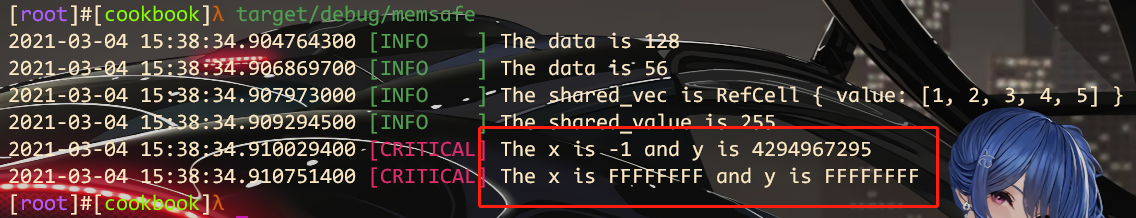
\includegraphics[width=\linewidth]{rust_raw_pointer.png}
  \caption{具有潜在错误的裸指针示例}
  \label{fig:rust_raw_pointer}
\end{figure}
x变成和y一样的值的原因在于:对指向y的指针类型做了转换,让它以为自己指向的是i64
类型,恰巧x就在y旁边,y被修改的同时,就顺带把x也修改了。因此,使用unsafe必须特别
小心。

在通常的情况下,虽然可以通过引用+mut的方式,可以阻止大部分的内存不安全问题,但是
由于引用+mut的强限制性,也为带来一些比较麻烦和无奈的问题,比如下面的代码:
\begin{code-block}{rust}
#[derive(Debug)]
struct Tuple {
    first: u8,
    second: u8,
    third: u8,
}
fn main() {
    let mut t = Tuple {
        first: 0,
        second: 1,
        third: 2,
    };
    let pa = &mut t.first;
    let pb = &mut t.second;
    let pc = &mut t.third;
    *pc += 10;
    info!("{:?}", t);
}
\end{code-block}
上述代码是正确无误的,可以正常编译和运行,但是,如果我们将结构体变成数组,问题就
出现了:
\begin{code-block}{rust}
fn main() {
    let mut array_x = [1_i32, 2, 8];
    let pa = &mut array_x[0];
    let pb = &mut array_x[1];
    *pb += 10;
    info!("{:?}", t);
}
\end{code-block}
上述代码在Rust 1.50.0版本之前就会出现错误:
\begin{code-block}{bash}
error: cannot borrow `x[..]` as mutable more than once at a time
\end{code-block}
原因在于,在Rust 1.50.0版本之前的结构体当中,pa,pb和pc指向不同的内存区域;
但是在数据当中,Rust编译器会将[\_]识别为一个整体,而\&[0], \&[1]之间都属于重叠,
将pa和pb判断为存在别名关系,即pa和pb实质上相同,违反了借用规则,因此无法通过编译。
采用引用分割才能进行解决:
\begin{code-block}{bash}
let mut array_x = [1_i32, 2, 3];
// 通过split_at_mut将数组切分成2个一定不会重叠的切片
let (first, rest): (&mut [i32], &mut [i32]) = array_x.split_at_mut(1);
let (second, third): (&mut [i32], &mut [i32]) = rest.split_at_mut(1);
first[0] += 100;
second[0] += 200;
third[0] += 300;
info!("{:?}", array_x);
\end{code-block}

由于Rust的目标是系统级的语言,必然需要具备操作硬件,以及裸设备的能力。而这些能力,
在C/C++的表述当中,通常是采用共用体(Union)实现的。为了与之兼容,Rust当中也引入了
Union数据结构,其主要的使用形式如下:
\begin{code-block}{rust}
#[repr(C)]
pub union U {
    pub i: u32,
    pub f: f32,
}

#[repr(C)]
pub struct Value {
    pub tag: u8,
    pub value: U,
}
\end{code-block}
其中,\#[repr(C)]必须使用,因为union的使用场景本身就是为了和C/C++进行对接,表示
该联合体使用和C/C++一样的内存布局。由于在字段当中使用了union,因此,结构体Value
也必须添加repr属性,否则会出现未定义的错误。而在使用的时候,则更加需要注意,只要
是涉及到读取联合体的字段,则必须使用unsafe:
\begin{code-block}{rust}
// 禁用illegal_floating_point_literal_pattern警告
#[allow(illegal_floating_point_literal_pattern)]
pub fn is_zero(v: &Value) -> bool {
    unsafe {
        match &v {
            Value {
                tag: Tag::I,
                value: U { i: 0 },
            } => true,
            Value {
                tag: Tag::F,
                // 会出现#[warn(illegal_floating_point_literal_pattern)]警告
                // 目前rust正在修复该问题
                value: U { f: 0.0 },
            } => true,
            _ => false,
        }
    }
}
\end{code-block}

Rust所有的unsafe实际都来源于性能和C的结合(比如写linux内核模块),因此原生指针
在unsafe当中最为常用。其主要的用途如下:
\begin{itemize}
  \item 在必要的时候跳过Rust安全检查:有的情况下,程序逻辑不会有任何内存安全的问题,原生指针可以跳过安全检查,提升性能
  \item 与C语言进行交互,必须使用原生指针
\end{itemize}

空指针在C语言当中非常常见,Rust当中也可以创建原生的空指针,也可以利用原生指针修改
数据:
\begin{code-block}{rust}
// 创建一个指向unsigned char的原生null指针
let pointer: *const u8 = std::ptr::null();
// 判断指针是否为空
assert!(pointer.is_null());

let mut s = [1, 2, 3];
// 创建一个可变的指针,该指针指向一个unsigned int的数组
let pointer: *mut u32 = s.as_mut_ptr();
assert!(!pointer.is_null());

unsafe {
    // 访问s[1]
    info!("The offset 1 is {}", *pointer.offset(1));
    // 访问s[2]
    info!("The offset 2 is {}", *pointer.offset(2));
    // 修改s[2]
    *pointer.offset(2) = 4;
    info!("The offset 2 is {}", *pointer.offset(2));
    // 将s[2]先转换成u8,然后再转换成char
    info!("The offset 2 is {}", *pointer.offset(2) as u8 as char);
}

info!("The final result of s is {:?}", s);
\end{code-block}

\section{杂项与技巧}

\subsection{预处理脚本与依赖关系}
在Rust当中,有的时候需要传递环境变量(编译期间)给源代码,生成特定的内容,此时
如果是直接在源代码当中进行环境变量的获取,则有可能获取到的是错误的信息。这种情况下
可以使用\colorblock{build.rs}脚本进行预处理。包含了该脚本的Rust工程结构大致如下:
\begin{figure}[H]
  \centering
  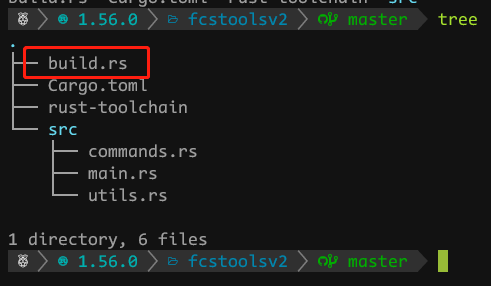
\includegraphics[width=\linewidth]{rust_build_rs.png}
  \caption{包含build.rs的工程结构}
  \label{fig:rust_build_rs}
\end{figure}

一个具体的build.rs实例如下:
\begin{code-block}{rust}
use std::process::Command;

fn main() {
    let output = Command::new("git")
        .args(&["rev-parse", "HEAD"])
        .output()
        .unwrap();
    let git_hash = String::from_utf8(output.stdout).unwrap();

    let __status__ = Command::new("git")
        .args(&["status", "--short"])
        .output()
        .unwrap();

    if "" != String::from_utf8(__status__.stdout).unwrap() {
        println!(
            "cargo:rustc-env=GIT_HASH={}-dirty",
            git_hash.trim_end_matches('\n')
        );
    } else {
        println!("cargo:rustc-env=GIT_HASH={}", git_hash);
    }
}
\end{code-block}

而在真正的源代码当中,使用则类似如下:
\begin{code-block}{rust}
...
let msg = format!(
    "For maintenance the AI Edge Platform, \nbuilt githash {}",
    env!("GIT_HASH"),
);
...
\end{code-block}

默认情况下,build.rs只会使用Rust标准库当中的所有函数和方法,即使是工程的Cargo.toml
文件的\codeinline{toml}{[dependencies]}引入了需要的依赖关系,build.rs仍然无法识别
相关的依赖包。如果需要在build.rs当中使用第三方的开发库,则需要修改工程的Cargo.toml
文件,添加如下的内容:
\begin{code-block}{rust}
# 表示给build.rs使用的依赖库
[build-dependencies]
chrono = "0.4.19"
\end{code-block}

注意,\codeinline{toml}{[dependencies]}和\codeinline{rust}{[build-dependencies]}当中
的依赖库是相互独立不影响的。如果build.rs当中的执行结果和预期的不一致,则可以直接
使用\codeinline{rust}{println!}进行输出打印,但是,这些信息不会在控制台上显示出来,
而是在\codeinline{bash}{target/xxx/build/yyy/output}当中,可以直接进行查看。

\section{常见错误处理方法}
由于很多代码都是第三方的,而Rust本身也在不断的发展,有可能出现版本不兼容或者特性
不兼容的情况,此时,则需要进行相关的修改。比如下面的一种错误:
\begin{figure}[H]
  \centering
  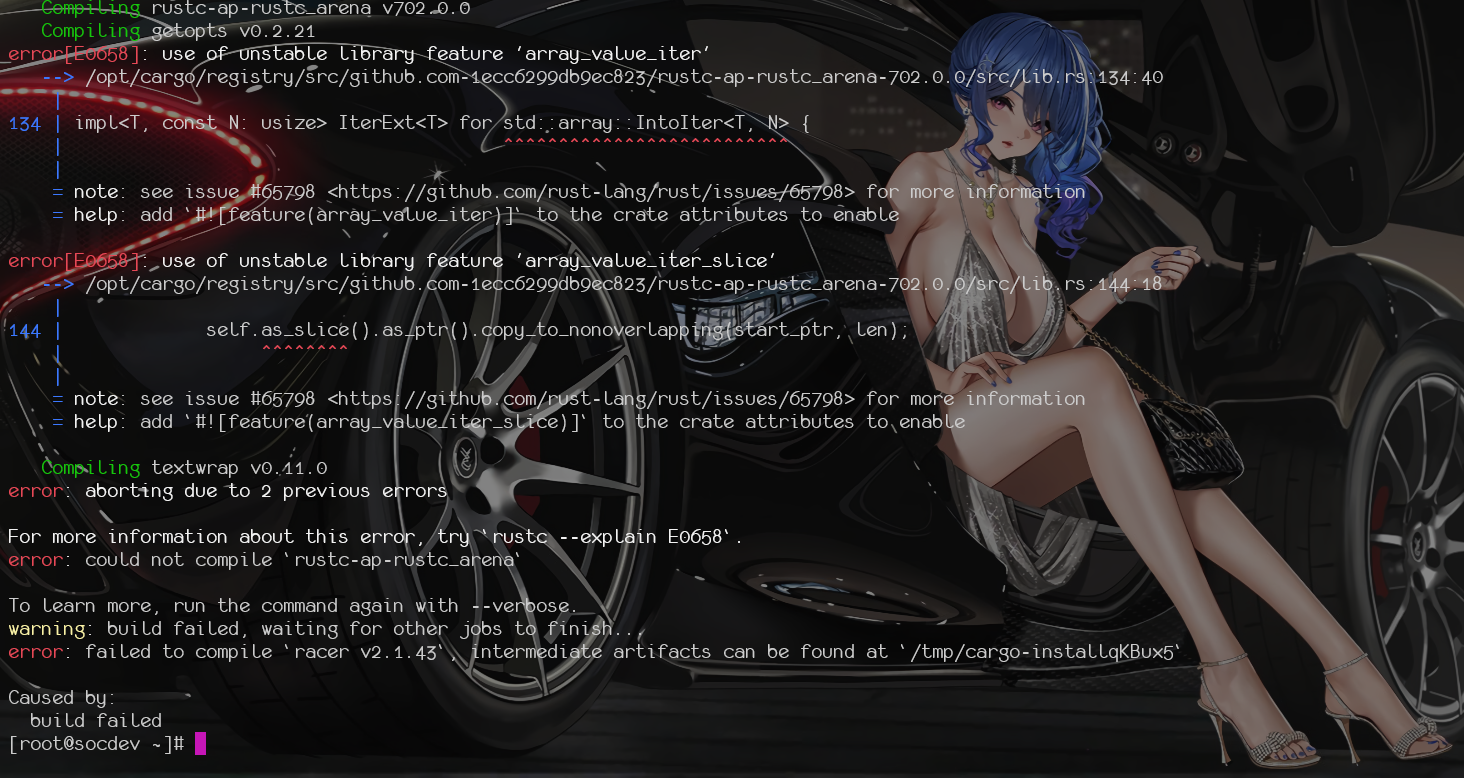
\includegraphics[width=\linewidth]{rust_feature_error.png}
  \caption{缺少特性支持编译失败}
  \label{fig:rust_feature_error}
\end{figure}
遇到这种错误,则需要直接修改对应的类库的源代码。以上述错误为例,编译的help表示
需要添加代码\codeinline{bash}{add `#![feature(array_value_iter_slice)]` to the crate attributes to enable},
则我们应当在对应的crate的lib.rs的头部当中,添加内容如下:
\begin{figure}[H]
  \centering
  
\includegraphics[width=\linewidth]{rust_feature_add.png}
  \caption{增加特性支持}
  \label{fig:rust_feature_add}
\end{figure}

\section{死灵书与实践}

\subsection{随机数实践}
Rust的随机数模块并不包含在标准库当中,需要使用rand这个crate,其基本的使用如下:
\begin{code-block}{rust}
use rand::distributions::{Distribution, Uniform};
use rand::seq::IteratorRandom;
use rand::Rng;
fn main() {
    let mut rng = rand::thread_rng();
    // 生成随机数
    info!("The float64 rand number is {}", rng.gen::<f64>());
    info!("The u32 rand number is {}", rng.gen::<u32>());
    info!("The i32 rand number is {}", rng.gen::<i32>());
    info!("The u8 rand number is {}", rng.gen::<u8>());
    // 从指定区间生成随机数
    info!("The range rand number is {}", rng.gen_range(0..100));
    info!(
        "The range rand float number is {}",
        rng.gen_range(10.0..50.0)
    );
    // 从[0, 5]生成随机数
    info!("The range rand number is {}", rng.gen_range(0..=5));
    // 定义[1, 7)的均匀分布
    let die = Uniform::from(1..7);
    // 从该分布当中生成采样
    let throw = die.sample(&mut rng);
    info!("The sample of uniform is {:>width$}", throw, width = 5);
    // 生成多个随机数
    let tuple: (u8, u8, u8) = rng.gen();
    info!("The tuple of random is {:?}", tuple);
    // 生成随机数组
    let array: [u8; 6] = rng.gen();
    info!("The array of random is {:?}", array);
    let mut exsit_array: [u8; 5] = [1, 2, 34, 5, 6];
    // 使用随机数填充已存在的数组
    rng.fill(&mut exsit_array);
    info!("The array of random is {:?}", exsit_array);
    // 从均匀分布当中随机采样3个数据
    // 得到的结果可能出现重复的情况
    let samples: Vec<u8> = (&mut rng).sample_iter(die).take(3).collect();
    info!("The samples of sample range 1..7 is {:?}", samples);
    let v = vec![1, 2, 3, 4, 5];
    // 从vec当中采样4个数据,得到的结果不会重复
    let sample = v.iter().choose_multiple(&mut rng, 4);
    info!("The samples of sample range 1..5 is {:?}", sample);
    let sample: Vec<u8> = (1..=10).choose_multiple(&mut rng, 4);
    info!("The samples of sample range 1..10 is {:?}", sample);
}
\end{code-block}

Rust的rand crate不仅可以生成随机数,也可以生成自定义的随机数据,比如:
\begin{code-block}{rust}
use rand::distributions::{Distribution, Standard, Uniform};
use rand::seq::IteratorRandom;
use rand::Rng;
struct Point {
    x: u8,
    y: u8,
}
impl fmt::Display for Point {
    fn fmt(&self, f: &mut fmt::Formatter) -> fmt::Result {
        write!(f, "x: {}, y: {}", self.x, self.y)
    }
}
// 在 Point 类型之上,对Standard实现Distribution trait,使得Point可以被gen函数随机生成
impl Distribution<Point> for Standard {
    // 默认的实现方法
    fn sample<R: Rng + ?Sized>(&self, rng: &mut R) -> Point {
        let (rand_x, rand_y) = rng.gen();
        Point {
            x: rand_x,
            y: rand_y,
        }
    }
}
fn main() {
    let mut rng = rand::thread_rng();
    let rand_point = rng.gen::<Point>();
    info!("The rand_point is {}", rand_point);
}
\end{code-block}

同样的,可以生成随机的字符串:
\begin{code-block}{rust}
use rand::distributions::{Alphanumeric, Distribution, Standard, Uniform};
use rand::seq::IteratorRandom;
use rand::Rng;
fn main() {
    let mut rng = rand::thread_rng();
    let rand_string: String = (&mut rng)
        // 从a-z,A-Z以及0-9当中进行选择
        .sample_iter(&Alphanumeric)
        // 获取其中的10个元素
        .take(10)
        // 默认的结果是char类型,需要继续转换成String
        .map(char::from)
        .collect();
    info!("The rand_string is {}", rand_string);
}
\end{code-block}

如果默认的字符集不满足要求,还可以自定义字符集,比如下面的示例:
\begin{code-block}{rust}
use rand::distributions::{Alphanumeric, Distribution, Standard, Uniform};
use rand::seq::IteratorRandom;
use rand::Rng;
const CHARSET: &[u8] = b"ABCDEFGHIJKLMNOPQRSTUVWXYZ\
    abcdefghijklmnopqrstuvwxyz\
    0123456789)(*&^%$#@!~";
const PASSWORD_LEN: usize = 10;
fn main() {
    let mut rng = rand::thread_rng();
    let password: String = (0..PASSWORD_LEN)
        .map(|_| {
            let idx = rng.gen_range(0..CHARSET.len());
            CHARSET[idx] as char
        })
        .collect();
    info!("The password is {}", password);
    // 也可以更换成之前的采样函数,看起来更为精炼
    let passwd: String = CHARSET
        .choose_multiple(&mut rng, 10)
        .map(|r| *r as char)
        .collect();
    info!("The password is {}", passwd);
}
\end{code-block}

同样的,针对自定义的数据类型,同样可以采用采样方法,进行随机数据的提取:
\begin{code-block}{rust}
use rand::distributions::{Alphanumeric, Distribution, Standard, Uniform};
use rand::seq::IteratorRandom;
use rand::Rng;
#[derive(Debug)]
struct Person {
    name: String,
    age: u8,
}
fn main() {
    let mut rng = rand::thread_rng();
    let persons = vec![
        Person {
            name: "lucifer".to_string(),
            age: 18,
        },
        Person {
            name: "titans".to_string(),
            age: 19,
        },
        Person {
            name: "garuda".to_string(),
            age: 36,
        },
    ];
    // 从person的vec当中,随机抽取2个元素
    let rand_person: Vec<_> = persons.choose_multiple(&mut rng, 2).collect();
    info!("The rand person is {:?}", rand_person);
}
\end{code-block}

\subsection{类型再论}
Rust的类型比较多,char,字符串,整数,浮点数等等。这些基础类型和其他语言比较类似,
但是也包含了自己的特点:比如,char类型占据4个字节,可以存放任何一个unicode字符;
对于ASCII字符,只需要一个字节即可,而一个字节的数据,则可以放在u8类型的数据当中,
因此,对于ASCII类型的字符串/字符数组,可以使用u8类型(即单字节)的数组进行存放,
这样,占用的资源空间会比char的数组小:
\begin{code-block}{rust}
fn main() {
    // 字符串前面的b,表示将对应的字面量存放在u8类型当中
    let s: &[u8] = b"hello";
    info!("{:?}", s);
}
\end{code-block}
同时,Rust支持的整数类型比较广泛,包括8bit,16bit,32bit,64bit,最大可以支持到
128bit;而特殊的isize和usize,则是和平台相关。如果平台是32位的,则isize和usize为
32位,如果是64位,则其数据宽度为64位。

整个Rust的类型当中,只有空类型占据的空间是最小的,都是0。Rust的空类型包括单元类型
(unit,即空元组)以及空结构体:
\begin{code-block}{rust}
// empty是空元组类型
let empty : () = ();
// 空结构体
struct Empty();
\end{code-block}
为了查看类型所占用的空间,可以使用size\_of函数进行查看:
\begin{code-block}{rust}
use std::mem;
struct Empty();
fn main() {
    info!("The Empty struct size is {}", mem::size_of::<Empty>());
    // 查看空元组所占据的内存大小
    info!("The none tuple size is {}", mem::size_of::<()>());
}
\end{code-block}

在Rust当中,浮点类型是非常特殊的数据类型。浮点类型当中,存在一个特殊的值:NaN,
即非法的浮点数值,因为该数据的存在,浮点数不具备全序关系(total order)。所谓的
全序,偏序,Rust当中的定义如下:对于集合X当中的元素a,b,c
\begin{itemize}
  \item 如果a<b,则!(a>b)一定成立;反之,如果a>b,则!(a<b)一定成立,即反对称性
  \item 如果a<b,b<c,则a<c,即传递性
  \item 对于X当中的所有元素,都存在a<b,或者a>b,或者a==b,三者必居其一,即完全性
\end{itemize}
如果X集合只满足前面2条,则称之为偏序;具备上述所有特征,则为全序。由于浮点数的NaN
不满足上述第3条规则,因此,Rust的浮点数属于偏序,而非全序,这回导致一个问题:浮点
数无法排序——非NaN的数值无法与NaN进行比较:
\begin{code-block}{rust}
let nan = std::f32::NAN;
let x = 0.4f32;
// 下列结果全部为false
info!("{}", nan > x);
info!("{}", nan < x);
info!("{}", nan == x);
\end{code-block}
为此,Rust设计了2个Trait表示全序与偏序:\codeinline{rust}{std::cmp::Ord}(全序)以及
\codeinline{rust}{std::cmd::PartialOrd}(偏序)。
PartialOrd这个Trait的partial\_cmp方法返回的是Option<Ordering>,而Ord返回的却是
Ordering。Rust的f32和f64都只实现了PartialOrd,因此,浮点类型无法进行排序,也同样无法
求取最值,如下列代码,则是无法运行的:
\begin{code-block}{rust}
let f_vec = vec![1f32, 2.0, 4.0, 0.0, -1.2];
let bigest_f = f_vec.iter().max();
\end{code-block}
对上诉代码进行编译,会直接提示如下类似的错误:
\begin{figure}[H]
  \centering
  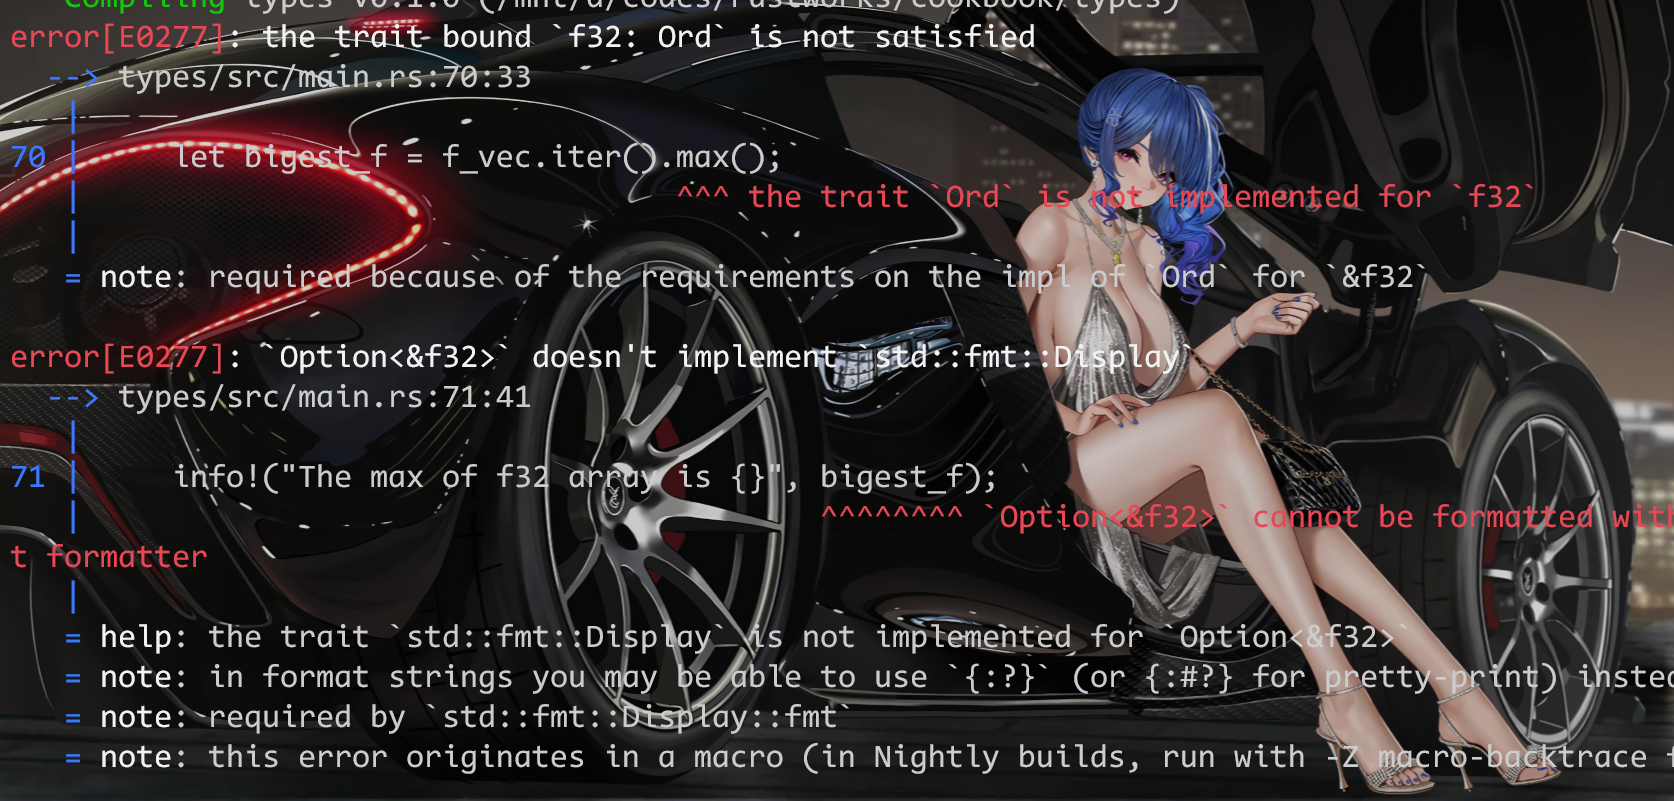
\includegraphics[scale=0.2]{rust_float_cmp_error.png}
  \caption{浮点数的最值错误求解}
  \label{fig:rust_float_cmp_error}
\end{figure}
浮点数的排序只能通过partial\_cmp(比较相等关系)进行变换处理,如下方代码:
\label{float_sort}
\begin{code-block}{rust}
let mut f_vec = vec![1f32, 2.0, 4.0, 0.0, -1.2];
// 升序排列
f_vec.sort_by(|first, second| first.partial_cmp(second).unwrap());
// 获取排序后的最后一位
let max = f_vec.last().unwrap();
// 或者如下进行
// let max = f_vec.as_slice().last().unwrap();
// 降序排列
f_vec.sort_by(|first, second| second.partial_cmp(first).unwrap());
\end{code-block}

作为常用数据类型之一,Rust的数组也存在自己的特点,比如同类型的数组之间可以相互赋值:
\begin{code-block}{rust}
let mut array: [u32; 4] = [1, 23, 4, 5];
let array_copy: [u32; 4] = [5, 6, 7, 8];
array = array_copy;
\end{code-block}
支持数组之间的直接比较,只是数组当中的元素本身就可以进行比较才行:
\begin{code-block}{rust}
let array: [u32; 4] = [1, 23, 4, 5];
let array_copy: [u32; 4] = [5, 6, 7, 8];
info!("{:?}", array < array_copy);
\end{code-block}

Rust当中的函数也可以称之为类型的一种,并且,每个函数都有自己单独的类型,函数的类型
是fn。但是,函数的参数列表会影响fn类型的判断和表达,比如下面的例子:
\begin{code-block}{rust}
fn add_tuple(t: (u32, u32)) -> u32 {
    t.0 + t.1
}
fn add_two((x, y): (u32, u32)) -> u32 {
    x + y
}
fn add_normal(x: u32, y: u32) -> u32 {
    x + y
}
\end{code-block}
实际上,add\_tuple和add\_two这2个函数被fn类型识别成为具有相同签名的类型,因此,
在理论上,我们可以使用同一个变量,接收这2个函数的指针:
\begin{code-block}{rust}
fn main() {
    let mut func = add_tuple;
    func = add_two;
    ...
}
\end{code-block}
但是,上述代码却是错误的:虽然签名相同,但是,类型不同:
\begin{figure}[H]
  \centering
  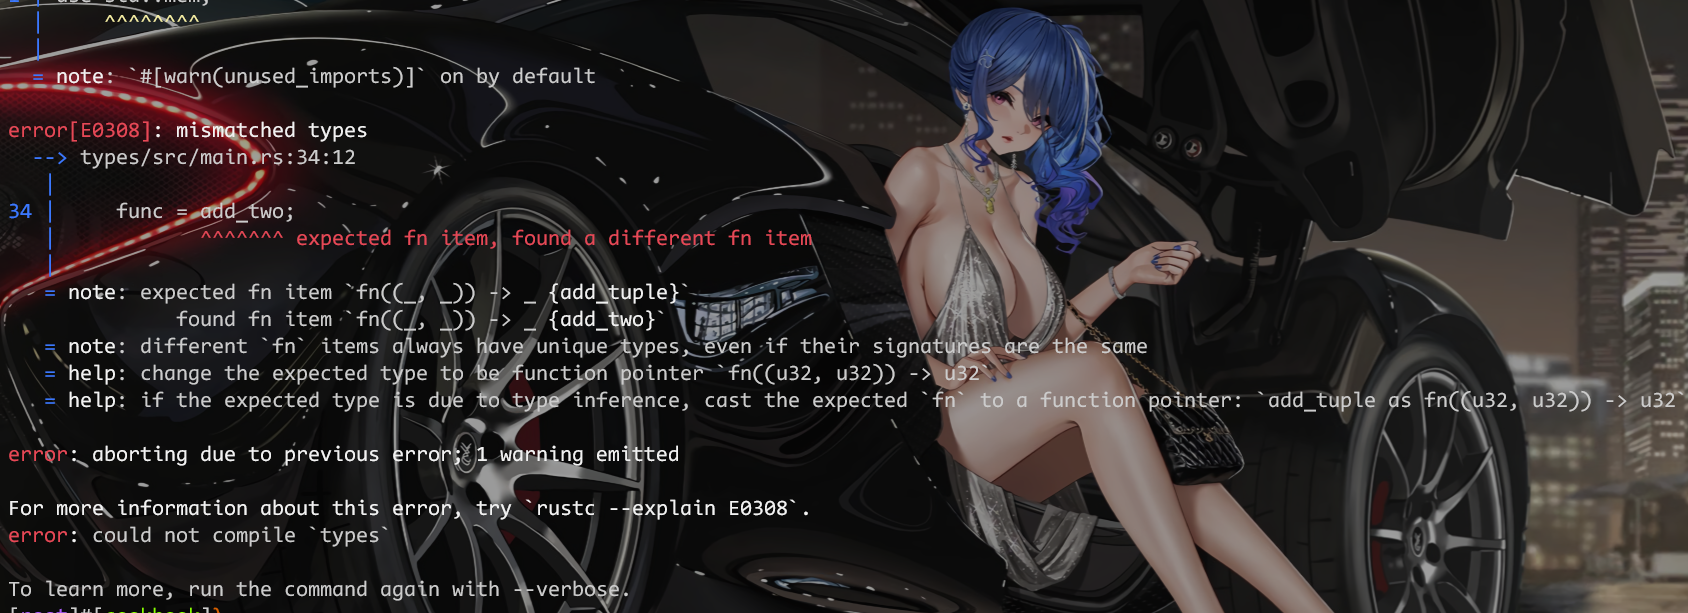
\includegraphics[width=\linewidth]{rust_func_type.png}
  \caption{相同签名的不同函数类型}
  \label{fig:rust_func_type}
\end{figure}
解决方法,则是将其转换成通用的fn类型:
\begin{code-block}{rust}
fn main() {
    // 显示指定func的类型
    let mut func: fn((u32, u32)) -> u32 = add_tuple;
    // 使用as进行类型的转换
    // let mut func = add_tuple as fn((u32, u32)) -> u32;
    func = add_two;
    ...
}
\end{code-block}
但是,需要注意,add\_normal的功能看上去和前面两个函数的功能相同,但是,他们的
函数签名完全不同,因此,不能将其转换成func。

函数是Rust的头等公民,可以在函数/方法当中定义函数,也可以在函数/方法当中定义结构
体,甚至于定义结构体的方法和实现,以及静态变量,常量等:
\begin{code-block}{rust}
fn func_as_first(x: u32, y: u32) -> (u32, u32) {
    struct Point {
        x: u32,
        y: u32,
    };
    impl Point {
        fn area(&self) -> u32 {
            self.x * self.y
        }
        fn cycle(&self) -> u32 {
            self.x + self.y
        }
    };
    let p = Point { x: x, y: y };
    (p.area(), p.cycle())
}
\end{code-block}

常规的函数类型,都会存在返回值,这些返回值要么是特定的类型,要么就是(),即类似
C/C++的返回void。如果需要什么都不返回,则可以使用!,这种函数称之为发散函数,比如
在处理panic时,有时就需要使用发散函数:
\begin{code-block}{rust}
fn diverges() -> ! {
    panic!("This function never returns!");
}
\end{code-block}
Panic操作会直接导致软件栈展开,因此,后续的操作都不会执行,其返回的就是一个!。
发散函数的最大特点,就是可以被转换成任意一个类型,虽然执行的时候最终还是会崩溃,
如下:
\begin{code-block}{rust}
let x : i32 = diverges();
let y : String = diverges();
\end{code-block}
但是,发散函数最大的作用,在于解决编译器的类型检查:
\begin{code-block}{rust}
let p = if x {
    panic!("error");
} else {
    100
};
\end{code-block}
对于let-if而言,if-else的每个分支都必须是相同的数据类型,通过发散函数的任意类型
转换特性即!与任何类型兼容,所以上述代码才能编译通过。

所有的Rust变量,函数都是类型的一种,都可以通过一定的手段和方式,获得类型的具体信息。
常见的方式有两种,一种是使用错误信息进行推断,一种则是使用标准库函数进行获得。

通过构造一个特殊的函数,然后调用该函数,则可以获得相关的类型信息:
\begin{code-block}{rust}
// 接收一个unit参数
fn type_id(_: ()) {}

fn main() {
    let ref i = 5;
    type_id(i);
}
\end{code-block}

而另外的方式,则是使用标准库函数,不过,这个标准库函数在Rust的默认stable分支当中
是不可用的,需要在nightly分支当中进行编译使用,并且,还需要启用一些特性:
\begin{code-block}{rust}
#![feature(core_intrinsics)]
use std;
// 使用泛型参数进行不同类型的数据接收
fn print_type<T>(_arg: &T) {
    println!(
        "The type name of arg is {}",
        std::intrinsics::type_name::<T>()
    );
}
fn main() {
    let ref x = 5;
    print_type(&x);
}
\end{code-block}
编译上述代码时,则需要对编译指令进行部分的调整:
\codeinline{bash}{cargo +nightly build},
然后即可实现对参数类型的打印输出。

在Rust当中,与Python不同,函数/方法并不存在默认参数,但是,结构体当中的字段,却可以
有默认值,只是,这个默认值的实现,必须和Default Trait相结合,如下:
\begin{code-block}{rust}
struct ColoredString {
    input: String,
    fg_color: String,
    bg_color: String,
}
impl Default for ColoredString {
    fn default() -> Self {
        ColoredString {
            input: String::default(),
            fg_color: String::default(),
            bg_color: String::default(),
        }
    }
}
fn main() {
    let color = ColoredString::default();
}
\end{code-block}
从上述代码当中可以看出,实际上,并不是Rust的结构体字段赋予了初始值,而是通过一个
名为default的方法,构造一个我们认为应该具有默认值的结构体。在Rust当中,常用的基本
数据类型都实现了Default Trait,可以直接使用对应的default方法。

\subsection{Trait类型与泛型再论}
关于类型,Trait也是比较重要的一个话题。在之前的示例当中,Trait全部是在具体的类型
上实现的,但是,Trait本身也可以在智能指针(Box)上实现,比如:
\begin{code-block}{rust}
trait Shape {
    fn area(self: Box<Self>) -> f64;
}
struct Circle {
    radius: f64,
}
impl Shape for Circle {
    fn area(self: Box<Self>) -> f64 {
        PI * self.radius * self.radius
    }
}
fn main() {
    let c = Box::new(Circle { radius: 4f64 });
    info!("{}", c.area());
    // 由于trait实现是在智能指针box上,因此,下面的使用是错误的
    // let c = Circle { radius: 4f64 }
    // c.area()
}
\end{code-block}
甚至在Trait上实现Trait,比如下方:
\begin{code-block}{rust}
trait Shape {
    fn area(&self) -> f64;
}
trait Round {
    fn get_radius(&self) -> f64;
}
struct Circle {
    radius: f64,
}
impl Round for Circle {
    fn get_radius(&self) -> f64 {
        self.radius
    }
}
impl Shape for dyn Round {
    fn area(&self) -> f64 {
        let radius = self.get_radius();
        PI * radius * radius
    }
}
\end{code-block}
Shape是一个Trait,Round同样也是一个Trait,Circle实现了Round,Round实现了Shape,
但是,由于Round本身是一个Trait,拥有不确定性,因此,在实现Shape的时候,需要添加
dyn关键字,提示这个Round不是普通的类型,而是一个Trait。上述代码当中,Circle间接
的实现了Shape,但是,Circle的类型无法直接使用Shape的方法,只能通过智能指针的方
式,将Circle转换成Round的类型,再进行使用,如下:
\begin{code-block}{rust}
fn main() {
    let c: Box<dyn Round> = Box::new(Circle { radius: 4f64 });
    info!("{}", c.area());
}
\end{code-block}
如果再把这个例子改得复杂一些,让Circle和Sphere同时实现Round,则我们可以使用Round
指针计算2个不同类型数据的结果:
\begin{code-block}{rust}
trait Shape {
    fn area(&self) -> f64;
}
trait Round {
    fn calc(&self) -> f64;
}
struct Circle {
    radius: f64,
}
impl Round for Circle {
    fn calc(&self) -> f64 {
        PI * self.radius * self.radius
    }
}
struct Sphere {
    radius: f64,
}
impl Round for Sphere {
    fn calc(&self) -> f64 {
        4f64 * PI * self.radius * self.radius
    }
}
impl Shape for dyn Round {
    fn area(&self) -> f64 {
        self.calc()
    }
}
fn main() {
    let circle: Box<dyn Round> = Box::new(Circle { radius: 4f64 });
    info!("The Circle area is {}", circle.area());
    let sphere: Box<dyn Round> = Box::new(Sphere { radius: 4f64 });
    info!("The Sphere area is {}", sphere.area());
}
\end{code-block}

Trait不仅仅用于实现类型,约束类型,还可以用于为其他现有的数据类型添加方法/函数,
比如:
\begin{code-block}{rust}
impl Round for i32 {
    fn calc(&self) -> f64 {
        *self as f64
    }
}
fn main() {
    let i_struct = 4i32;
    i_struct.calc();
}
\end{code-block}
这种类型的函数/方法,则称之为扩展方法/函数。从上述例子当中,我们似乎可以使用Trait
对任意类型进行函数/方法的扩展,但是,这个是存在前提的:
\begin{itemize}
  \item impl和trait的声明/定义在同一个crate当中
  \item 或者,impl的实现需要和类型的声明在同一个crate当中
\end{itemize}
如果不满足上述条件,则容易出现bug和问题,也会违反Rust的规则。

Rust的Trait支持多种特性,自然也支持继承,但是注意,Rust的结构体和enum数据类型并不
存在继承的概念。Trait的继承方式如下:
\begin{code-block}{rust}
trait Base {}
trait Derived : Base {}
\end{code-block}
当一个结构体实现了上述的Derived这个Trait,则必须同样实现Base这个Trait,否则就会
出现语法错误:
\begin{code-block}{rust}
trait Base {}
trait Derived : Base {}
struct T;
impl Derived for T {}
impl Base for T {}
\end{code-block}

Rust的Trait不仅可以包括函数的定义,同样可以直接定义函数:
\begin{code-block}{rust}
trait Page {
    fn set_page(&self) {
        info!("Page Default: 1");
    }
}
trait PerPage {
    fn set_per_page(&self) {
        info!("Per Page Default: 1");
    }
}
struct Paginate {
    page: u32,
}
impl Page for Paginate {}
impl PerPage for Paginate {}
fn main() {
    let page = Paginate { page: 8 };
    page.set_page();
    page.set_per_page();
    page.set_skip_page();
}
\end{code-block}

甚至于,Trait可以直接给结构体提供更多的组合方法:
\begin{code-block}{rust}
trait PaginateMore: Page + PerPage {
    fn set_skip_page(&self) {
        info!("Skip the page");
    }
}
fn main() {
    ...
    page.set_skip_page();
}
\end{code-block}
结构体根本不用自行实现Trait PaginateMore,就可以直接使用该Trait当中的方法。

Trait不仅仅可以用于接口实现,在Rust当中,更重要的则是类型限定,限定某些数据只能
做某些事情。比如下方的代码:
\begin{code-block}{rust}
...
fn static_dispatch<T>(t: &T) where T: Bar {
    ...
}
fn dynamic_dispatch(t : &Bar) {
    ...
}
\end{code-block}
对于实现了Trait Bar的类型来说,上述2个函数,都可以被调用,但是,从语法上,static\_dispatch
由于使用了where,表示参数必须限定在Trait Bar类型,在编译时就能够确定;而dynamic\_dispatch
则从语法上表示,输入的参数必须是Bar的对象,即Trait Object。运行时,Trait Object会根据虚表
指针从虚表当中查出正确的指针,再进行动态调用,属于在运行时确定。

但是并不是每一个Trait都可以当着Trait Object使用,这个和类型大小是否确定有关系。每一个
Trait的隐藏类型参数Self默认限定为?Sized,?Sized trait包括了所有动态大小类型以及所有
可确定大小的类型。Rust当中大部分类型都是默认可确定大小的,即<T:Sized>。当trait对象
在运行期进行动态分发时,也必须确定大小,否则无法分配内存。只有同时满足下列条件的
trait,才可以当作Trait Object使用:
\begin{itemize}
  \item Trait的Self不能被限定为Sized
  \item Trait当中的所有方法都必须是对象安全的
\end{itemize}

而所谓的对象安全,则必须满足如下的条件\colorblock{之一}:
\begin{itemize}
  \item 当Trait的Self被限定为Sized时,方法受Self:Sized约束
  \item Trait的方法签名必须\colorblock{同时满足以下3点}
  \begin{enumerate}
    \item 不包含任何泛型参数(Self)
    \item 第一个参数必须为Self类型或可解引用为Self类型
    \item Self不能出现在除第一个参数之外的其他地方
  \end{enumerate}
  \item Trait当中不能包含关联常量
\end{itemize}

比如下面的代码,就属于标准的对象安全:
\begin{code-block}{rust}
trait Bar {
    fn bax(self, x: u32);
    fn bay(&self);
    fn baz(&mut self);
}
\end{code-block}
Trait Bar不受Sized限制,Trait的方法没有额外的Self类型参数,没有泛型参数,因此是安全的。
相对应的,不安全的Trait如下:
\begin{code-block}{rust}
// 对象不安全
trait Foo {
    fn bad<T>(&self, x:T);
    fn new() -> Self;
}
// 对象安全
trait Foo {
    fn bad<T>(&self, x: T);
    fn new() -> Self
    where
        Self: Sized;
}
\end{code-block}

当然,Sized约束也可以用于Trait定义当中。比如,自行实现一个类似any的Any Trait。
\begin{code-block}{rust}
use std::ops::Fn;
trait CustomAny {
    fn custom_any<F>(&self, f: F) -> bool
    where
        Self: Sized,
        F: Fn(u32) -> bool;
}
impl CustomAny for Vec<u32> {
    fn custom_any<F>(&self, f: F) -> bool
    where
        Self: Sized,
        F: Fn(u32) -> bool,
    {
        for &x in self {
            if f(x) {
                return true;
            }
        }
        false
    }
}
fn main() {
    let v: Vec<u32> = vec![1, 2, 3];
    info!("{}", v.iter().any(|&x| x == 3));
    info!("{}", v.custom_any(|x| x == 3));
}
\end{code-block}

Trait当中不仅可以包含函数和方法,同样可以包含变量和常量,即所谓的关联变量以及关联
常量。关联常量的使用稍微有些特殊,在Trait当中可以定义关联常量,但是,使用的时候,
却是通过Trait的实现对象来使用这些关联常量的:
\begin{code-block}{rust}
trait Colorize {
    // 定义关联常量
    const FG_RED: &'static str = "31";
    const BG_YELLOW: &'static str = "43";
    fn red(self) -> ColoredString;
    fn on_yellow(self) -> ColoredString;
}
impl Colorize for ColoredString {
    fn red(self) -> ColoredString {
        ColoredString {
            // 使用关联常量,如果是Colorize::FG_RED,则会提示错误
            fg_color: String::from(ColoredString::FG_RED),
            ..self
        }
    }
    fn on_yellow(self) -> ColoredString {
        ColoredString {
            bg_color: String::from(ColoredString::BG_YELLOW),
            ..self
        }
    }
}
\end{code-block}

Trait不仅仅可以实现泛型,泛型也不仅限于Trait和<T>,对于函数/方法,也可以使用在
泛型、生命周期以及Trait当中,比如,显式的指定闭包的生命周期:
\begin{code-block}{rust}
// 将函数作为泛型参数
struct Pick<F> {
    data: (u32, u32),
    func: F,
}
impl<F> Pick<F>
where
    // for<>只能用于标记生命周期
    F: for<'f> Fn(&'f (u32, u32)) -> &'f u32,
{
    fn call(&self) -> &u32 {
        (self.func)(&self.data)
    }
}

fn max(data: &(u32, u32)) -> &u32 {
    if data.0 > data.1 {
        return &data.0;
    }
    &data.1
}
fn main() {
    let pick = Pick {
        data: (32, 34),
        func: max,
    };
    info!("{}", pick.call());
}
\end{code-block}

\subsection{常见的设计模式}
建造者模式是Rust当中最常用的设计模式之一,其主旨思想在于将可变和不可变进行分离,
一种基本的示例如下:
\begin{code-block}{rust}
use std::f64::consts;
pub struct Circle {
    radius: f64,
}
pub struct CircleBuilder {
    radius: f64,
}
impl Circle {
    pub fn new() -> CircleBuilder {
        CircleBuilder { radius: 0.0 }
    }
    pub fn area(&self) -> f64 {
        self.radius * self.radius * consts::PI
    }
}
impl CircleBuilder {
    pub fn radius(&mut self, radius: f64) -> &mut CircleBuilder {
        self.radius = radius;
        self
    }
    pub fn build(&self) -> Circle {
        Circle {
            radius: self.radius,
        }
    }
}
\end{code-block}

\subsection{排序}
Rust的整数型数组和向量(Vector)的排序是相同的,可以使用相同的方式进行,即采用
sort以及sort\_unstable进行。其中,sort是稳定排序(即不重新排序相等的元素),
sort\_unstable是不稳定排序,\colorblock{但是通常情况下速度更快},并且不会进行辅助内存的分配。
\begin{code-block}{rust}
let mut v = vec![2, 21, 12, 32, 12, 45, 90];
v.sort_unstable();
info!("The sorted vector is {:?}", v);
let mut array = [2, 23, 12, 12, 98, 100, 21];
array.sort_unstable();
info!("The sorted array is {:?}", array);
\end{code-block}
默认情况下,排序操作使用的是升序,但是可以通过定制,修改排序方式:
\begin{code-block}{rust}
let mut v = vec![2, 21, 12, 32, 12, 45, 90];
// 降序排列,可替换成v.sort_by
v.sort_unstable_by(|a, b| b.cmp(a));
info!("The sorted vector is {:?}", v);
let mut array = [2i32, -23, 12, 12, 98, -100, 21];
// 根据绝对值升序排列,可以根据其他关键字进行排序
array.sort_unstable_by_key(|k| k.abs());
info!("The sorted array is {:?}", array);
// 根据字符顺序排列,带有缓存cache,闭包函数通常只执行一次,比无缓存的快速
let mut xx = [-5i32, 4, 32, -3, 2];
xx.sort_by_cached_key(|k| k.to_string());
// 字符串排序
let mut array = ["lucifer", "titans", "asura", "garuda"];
array.sort_unstable_by_key(|item| item.to_string());
info!("The string array is {:?}", array);
let mut array = [
    "lucifer".to_string(),
    "titans".to_string(),
    "asura".to_string(),
    "garuda".to_string(),
];
// 可以转换成切片
// array[..].sort_unstable_by_key(|item| item.to_string());
// info!("The string array is {:?}", array);
array.sort_unstable_by_key(|item| item.to_string());
info!("The string array is {:?}", array);
\end{code-block}

浮点数的排序和最值操作,参见\colorunderlineref{float_sort}

除了基础数据类型可以进行排序,同样可以针对复合数据类型进行排序。在针对复合数据
类型排序时,需要实现\colorblock{Eq,PartialEq,Ord和PartialOrd}这几个trait:
\begin{code-block}{rust}
#[derive(Eq, PartialEq, Ord, PartialOrd, Debug)]
struct Student {
    name: String,
    age: u8,
}
fn main() {
    let mut stu = [
        Student {
            name: "lucifer".to_string(),
            age: 18,
        },
        Student {
            name: "garuda".to_string(),
            age: 36,
        },
    ];
    // 按照自然序列(name)
    stu.sort();
    info!("The students is {:?}", stu);
    // 根据年龄
    stu.sort_unstable_by(|first, second| first.age.cmp(&second.age));
    info!("The students is {:?}", stu);
}
\end{code-block}

\subsection{压缩与解压}
Rust可以实现文件的压缩与解压,在Linux环境下,通常使用\href{https://github.com/alexcrichton/tar-rs}{tar}(归档)
和\href{https://github.com/rust-lang/flate2-rs}{flate2}(压缩解压),比如Linux下常见的tar.gz文件的处理:
\begin{code-block}{rust}
use flate2::read::GzDecoder;
use flate2::write::GzEncoder;
use flate2::Compression;
use tar::Archive;

let path = "/root/py3.tar.gz";
let targz = match File::open(path) {
    Ok(file) => file,
    Err(error) => {
        crit!("Failed to open the file {}: {}", path, error.to_string());
    }
};
// gz文件的解码器
let tar = GzDecoder::new(targz);
// tar的管理器
let mut archive = Archive::new(tar);
// 将tar.gz解压
match archive.unpack(".") {
    Ok(_) => info!("Sucess to unpack the tar.gz file"),
    Err(error) => {
        crit!("Failed to unpark the tar.gz file: {:?}", error);
    }
}
// 创建tar.gz文件
let targz = match File::create("log.tar.gz") {
    Ok(file) => file,
    Err(error) => {
        crit!(
            "Failed to create the log.tar.gz file : {}",
            error.to_string()
        );
    }
};
// 创建gz文件的编码器,压缩算法使用默认
let encoder = GzEncoder::new(targz, Compression::default());
let mut tarfile = tar::Builder::new(encoder);
// 将文件添加到tar.gz文件当中
match tarfile.append_dir_all("log", "/var/log") {
    Ok(_) => info!("log.tar.gz created sucessful"),
    Err(error) => {
        fs::remove_file("log.tar.gz").unwrap_or_else(|why| {
            error!("Cannot remove the log.tar.gz: {:?}", why.to_string())
        });
        crit!("Failed to park the tar.gz file: {:?}", error);
    }
}
\end{code-block}

当然,归档和压缩也可以单独使用:
\begin{code-block}{rust}
use flate2::read::GzDecoder;
use flate2::write::GzEncoder;
use flate2::Compression;
use tar::Archive;
let tarf = match File::create("log.tar") {
    Ok(file) => file,
    Err(error) => {
        crit!("Failed to create the log.tar file : {}", error.to_string());
    }
};
// 注意和gz文件不一样,只是归档,则不需要创建编码器
let mut tar_file = tar::Builder::new(tarf);
match tar_file.append_dir_all("log", "/var/log") {
    Ok(_) => info!("log.tar created sucessful"),
    Err(error) => {
        fs::remove_file("log.tar")
            .unwrap_or_else(|why| error!("Cannot remove the log.tar: {:?}", why.to_string()));
        crit!("Failed to park the tar.gz file: {:?}", error);
    }
}
let path = "/root/log.tar";
let tarball = match File::open(path) {
    Ok(file) => file,
    Err(error) => {
        crit!("Failed to open the file {}: {}", path, error.to_string());
    }
};
// 同样的,解压tar文件,不需要创建解码器
let mut archive = Archive::new(tarball);
match archive.unpack(".") {
    Ok(_) => info!("Sucess to unpack the tar file"),
    Err(error) => {
        crit!("Failed to unpark the tar file: {:?}", error);
    }
}
\end{code-block}

